\documentclass[12pt, a4paper, oneside]{report}
\usepackage[utf8]{inputenc}
\usepackage[catalan]{babel}
\usepackage{titlesec}
\usepackage{lipsum}
\usepackage{setspace}
\usepackage[Glenn]{fncychap}
\usepackage[a4paper,left=0.8in,right=0.8in,top=1.2in,bottom=1.2in]{geometry}
\usepackage{xcolor}
\usepackage{blindtext}
\usepackage[skip=13pt]{parskip}
\usepackage{enumitem}
\usepackage{minted}
\usepackage{graphicx}
\usepackage{amsfonts}
\usepackage{pdfpages}
\usepackage{verbatim}
\usepackage{appendix}
\usepackage{pgfplots}
\usepackage{xpatch}
\usepackage{fancyhdr}
\usepackage{wrapfig}
\usepackage{parskip}
\usepackage{needspace}
\usepackage[labelfont=bf]{caption}
\usepackage{titlesec}
\usepackage[bottom]{footmisc}
\usepackage{subfig}
\usepackage{caption}
% \usepackage{subcaption}
\usepackage{diagbox}
\usepackage{helvet}
\usepackage{hyperref}
\usepackage{mdframed}

% \newenvironment{longlisting}{\captionsetup{type=listing}}{}
\newenvironment{longlisting}{\captionsetup{type=figure}}{}

\hypersetup{
    colorlinks,
    linkcolor={black},
    % citecolor={blue!50!black},
    urlcolor={blue!80!black}
}

\newcommand{\nocontentsline}[3]{}
\newcommand{\tocless}[2]{\bgroup\let\addcontentsline=\nocontentsline#1{#2}\egroup}

\captionsetup{font=footnotesize}

\definecolor{LightGray}{gray}{0.95}
\setlist{nosep} %espai entre llistes
\newcommand{\quotes}[1]{``#1''}

%afegeix colors al text r4
\definecolor{vermellpral}{RGB}{207, 16, 32} % #CF1020
\definecolor{blau}{RGB}{0, 96, 240}
\definecolor{taronja}{RGB}{255, 136, 73}
\definecolor{verd}{RGB}{105, 190, 40}

\renewcommand{\baselinestretch}{1.5} %espaiat 1.5

%canviar colors de les capçaleres dels capitols r3
\xpatchcmd\DOCH
  {\mghrulefill}{\color{vermellpral}\mghrulefill}
  {}{\PatchFailed}
  \ChTitleVar{\bfseries\Large\rmfamily\scshape\color{black}}
  \ChNameVar{\bfseries\Large\rmfamily\color{black}}
\xpatchcmd\DOTIS
  {\mghrulefill}{\color{vermellpral}\mghrulefill}
  {}{\PatchFailed}

\title{TdR}
\author{Jordina Gavaldà Rovira}
\date{April 2022}

% capçalera
\pagestyle{fancy}
%\rhead{\thepage}
\rhead{}
\lhead{}
\chead{\leftmark}
\cfoot{\thepage}
\let\HeadRule\headrule
\renewcommand\headrule{\color{vermellpral}\HeadRule} %color capçalera
\setlength{\headheight}{15.71667pt}

% change part format for annex
\titleformat{\part}[display]
{\normalfont\Large\bfseries}{}{0pt}{\Large\thepart\hskip1em}
\titleformat{name=\part,numberless}[display]
{\normalfont\Large\bfseries}{}{0pt}{\Large}
\titlespacing*{\part}{0pt}{0pt}{0pt}
\titlespacing*{name=\part,numberless}{0pt}{0pt}{0pt}
\renewcommand{\thepart}{\arabic{part}}
\titleclass{\part}{straight}

\newenvironment{example}{%
\begin{list}{}{%
\setlength{\leftmargin}{1cm}%
\setlength{\rightmargin}{1cm}%
\setlength{\listparindent}{\parindent}%
\setlength{\itemindent}{\parindent}%
\setlength{\parsep}{\parskip}%
\sffamily
}%
\item[]}{\end{list}}

\begin{document} %--------------------------------------------------------------------------


\includepdf[pages={1}]{capitols/figures/coberta.pdf}

\pagestyle{empty}
\tableofcontents
\addtocontents{toc}{\protect\thispagestyle{empty}}

\newpage

\pagestyle{fancy}

\listoffigures

\chapter*{Abstract}
\addcontentsline{toc}{chapter}{Abstract}
\markboth{ABSTRACT}{}
Technology is evolving very rapidly and competition between companies is fierce. They want their devices to be the safest, fastest and most efficient. In order to achieve that, they need very good hardware and software. The programs, procedures and routines that make up the software must be developed very carefully to be as efficient as possible. To further analyze these programs and procedures, we need to study the process they perform without considering the implementation. In other words, we need to study the algorithm they use to solve a particular computational problem.

In this paper we will study what algorithms are and how their time efficiency is analyzed. Then, two search algorithms and two sorting algorithms will be analyzed theoretically and practically and the results obtained will be compared. We will also briefly talk about algorithmic analysis when using nonlinear data structures. Finally, to visualize the algorithms, I have created two programs: one for sorting and searching algorithms and the other for pathfinding algorithms.

\textit{Keywords}: algorithm, array, BFS, Big O notation, binary search, bubble sort, complexity, DFS, Dijkstra, efficiency, graphs, hardware, input, latex, linear search, merge sort, output, practical analysis, program, running time, searching, software, sorting, theoretical analysis, visualization.

\chapter*{Introducció}
\addcontentsline{toc}{chapter}{Introducció}
\markboth{INTRODUCCIÓ}{}
\section*{Justificació del treball}
\addcontentsline{toc}{section}{Justificació del treball}
Vivim en una societat en la qual utilitzem dispositius electrònics per a tot. Per a comunicar-nos, treballar, oci, estudiar, jugar, comprar... I quan hi ha molta demanda d'aquests dispositius, es busca optimitzar-los, fer-los més agradables per l'usuari i fer-los més ràpids.

Estar clar que és més còmode esperar menys a què s'encengui l'ordinador, obrir més ràpidament les aplicacions del mòbil, i, per tant, consumir menys bateria. O buscar un fitxer i trobar-lo en segons en lloc de minuts, actualitzar el sistema en menys temps, fer una cerca a internet i tardar mil·lèsimes de segon... Si el treball de l'usuari es troba interromput a causa del dispositiu, està clar que l'usuari no haurà tingut una bona experiència i evitarà fer ús d'aquesta eina.

Hi ha diverses formes de fer un dispositiu més ràpid, òbviament utilitzant millors components tindrem un millor dispositiu, però el preu també serà molt superior. També és molt important la programació del dispositiu, tant del sistema operatiu com de les aplicacions. No serveix de res tenir el millor dispositiu si a l'hora de fer la feina el programa no és eficient. No s'estaria utilitzant el màxim potencial dels components. A més, té el mateix cost programar-ho millor o pitjor, per això és tan important optimitzar-ho al màxim per crear un dispositiu eficient, de qualitat i assequible.

Personalment, des de fa un parell d'anys participo en concursos de programació, aquests consisteixen en resoldre problemes de matemàtiques en què la solució és un programa. Aquesta solució ha de resoldre el problema de la forma més eficient possible, i sempre s'utilitzen algoritmes.

En aquest treball ens centrarem en la part de programar de forma eficient, i per simplificar-ho i entendre bé els conceptes, utilitzaré alguns problemes dels concursos com a exemples.

\section*{Objectius}
\addcontentsline{toc}{section}{Objectius}
En aquest projecte podem definir dos tipus d'objectius, els que fan referència al contingut del treball:
\begin{itemize}
    \item Estudiar i definir que és l'algorísmia i per a què serveix. 
    \item Estudiar com s'analitza i compara l'eficiència dels algoritmes i programes.
    \item Estudiar i comparar de forma teòrica alguns algoritmes.
    \item Implementar aquells algoritmes i comparar de forma pràctica els programes.
    \item Realitzar un programa per visualitzar els algoritmes estudiats.
\end{itemize}
I els que fan referència a la realització del treball:
\begin{itemize}
    \item Realitzar un treball amb el programari Overleaf i \LaTeX.
\end{itemize}

LaTeX és un sistema de composició de textos, orientat especialment a la creació de llibres, documents científics i tècnics que continguin fórmules matemàtiques. 

Overleaf és un editor en línia de \LaTeX. 


\section*{Metodologia}
\addcontentsline{toc}{section}{Metodologia}
Per assolir els nostres objectius, partirem el treball en dues parts teòriques i dues parts pràctiques: En la primera part teòrica, definirem tots els conceptes importants, explicarem que és un algoritme, per què són importants, i com s'analitzen per poder determinar quin és l'òptim. 

En la segona part teòrica posarem exemples més concrets i els analitzarem per poder predir el seu comportament en diferents situacions. 

En la primera part pràctica implementarem els algoritmes de la segona part teòrica, i compararem els resultats teòrics amb els pràctics. També implementarem una visualització dels algoritmes.

I finalment, acabarem editant aquest treball en el llenguatge \LaTeX.

\setcounter{chapter}{0}
\chapter{Conceptes bàsics} 

\section{Com funcionen els dispositius electrònics}
Els dispositius electrònics com els telèfons mòbils, tauletes, ordinadors, caixers automàtics, consoles, impressores, rentaplats, televisions, rentadores, microones, robots, ràdios... tots resolen tasques diferents, i tenen utilitats diferents, però tots funcionen fonamentalment de la mateixa manera. 

\subsection{Com interactuem amb els dispositius electrònics}
Els dispositius són màquines que responen a accions com ara tocar la pantalla tàctil, clicar amb el ratolí, escriure amb el teclat, parlar pel micròfon, prémer algun botó del comandament a distància... i, el dispositiu et genera una resposta en funció de l'acció que hagis fet: pot canviar el contingut de la pantalla, reproduir un so a través dels altaveus, enviar un senyal a un altre dispositiu, canviar el canal de la televisió, retirar una quantitat de diners...

La informació que dones al dispositiu l'anomenarem \textbf{entrada}. I al resultat o resposta que et genera l'anomenarem \textbf{sortida}. 

Per exemple, quan premem el botó d'apujar el volum del comandament de la televisió, estàs generant una entrada. La televisió la processa i genera una sortida en funció de l'entrada, és a dir, apuja el volum. Si l'entrada fos diferent i haguéssim premut el botó de canviar de canal, la sortida també seria diferent, i s'hauria canviat el canal en lloc d'apujar el volum. Podem deduir doncs que la sortida depèn completament de l'entrada. Si canviem l'entrada, la sortida també serà diferent.

Els components de l'ordinador en si no poden processar les entrades i generar sortides, es necessita algun element que rebi la informació (entrada), la processi i generi el resultat (sortida). Aquí és on entra la programació. Els programes processen la informació i donen les ordres als components per generar una sortida.

Per exemple, premem el botó d'engegar del mòbil (entrada), l'entrada arriba al programa, aquest processa la informació i genera una sortida, la qual consisteix a encendre la pantalla del mòbil.

\begin{figure}[h]
    \centering
    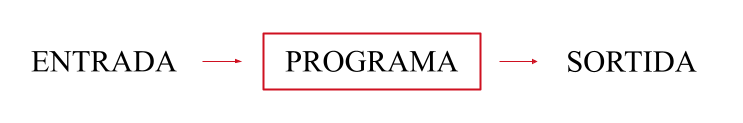
\includegraphics[width=.7\textwidth]{capitols/figures/i_o prog.png}
    \caption[Diagrama d'entrada, programa i sortida.]{Diagrama d'entrada, programa i sortida. Font: elaboració pròpia.}
    \label{Figura}
\end{figure}

Totes les tasques que podem resoldre utilitzant un programa les anomenarem problema. Ens referim a tots els exemples d'aquest punt com a un problema que hem resolt amb un programa. 

Quan parlem d'un problema matemàtic com ara sumar dos nombres, la solució és el resultat de la suma, l'equivalent a la sortida. Però quan parlem de problemes de programació, com els d'aquest treball, la solució és el procediment, el qual és diferent de la sortida, ja que la sortida és el resultat de finalitzar el procediment.

\subsection{Que són els algoritmes i en què es diferencien dels programes}
Un algoritme és un procediment, un seguit de passos finits i ordenats que resolen una tasca o problema concret. Els algoritmes ofereixen formes teòriques de resoldre un problema.

% treure llenguatge de programació
En canvi, un programa és tot allò que un ordinador pot entendre i executar. Un programa pot implementar\footnote{La paraula 'implementar' s'utilitza en aquest context per expressar l'acció de passar alguna solució/procediment/algoritme a un programa. La implementació d'un algoritme és un programa que resolgui la mateixa tasca que l'algoritme implementat.} o \quotes{traduir} un algoritme. Els programes ofereixen formes pràctiques de resoldre un problema.

És a dir, els algoritmes són el procediment o els passos a seguir. I els programes són la traducció dels algoritmes de manera que els ordinadors ho puguin entendre i executar.
%traduir
% Aquests conceptes que he explicat fins ara ens els trobem diàriament. Per exemple, quan volem cuinar un plat de pasta, necessitem diversos elements: ingredients, una recepta i un cuiner. Amb la recepta tenim la teoria de com hem de cuinar per tenir el plat de pasta, el cuiner executa la recepta, i depenent del tipus de pasta que utilitzi obtindrà plats diferents. Si la recepta diu que s'han d'utilitzar macarrons, només podràs fer un plat de macarrons. En canvi, si diu que es pot utilitzar qualsevol classe de pasta, podràs seguir aquesta recepta tant per fer espaguetis com macarrons.

% Amb els ordinadors passa el mateix. Quan volem resoldre un problema com cuinar un plat de pasta, necessitem: entrades, un algoritme i un programa. Amb l'algoritme (recepta) tenim la teoria de com resoldre el problema, el programa seria el cuiner, ja que aplica l'algoritme o teoria i resol el problema a la pràctica. Finalment, les entrades serien els ingredients, i depenent de les entrades obtindrem diferents sortides, igual que amb diferents tipus de pasta podem obtenir diferents plats o sortides. Podem seguir la mateixa recepta amb diferents tipus de pasta i, per tant, el cuiner farà el mateix. Igual que pots utilitzar el mateix algoritme i programa amb diferents entrades i la sortida dependrà de l'entrada. Ja que si cuines amb macarrons, no obtindràs espaguetis.

Per exemple, hi ha el següent problema que volem resoldre amb un programa: agafem tres nombres que anomenem $x, y, z$ i volem trobar $(x+y)\cdot z$. Aquest problema està generalitzat perquè no tenim valors fixos per l'entrada i, per tant, no podem saber quina és la sortida. És a dir, farem un algoritme i programa que funcionin per a qualsevol nombre, no només un.

Per solucionar matemàticament aquest problema, primer cal resoldre la suma, i després la multiplicació. I per fer un programa que el resolgui, podríem fer el següent:

ALGORITME:
\begin{enumerate}
    \item Llegir els nombres amb l'ordre adequat.
    \item Sumar els dos primers nombres.
    \item Multiplicar el resultat del pas 2 pel tercer nombre.
    \item La solució és el resultat del pas 3.
\end{enumerate}

PROGRAMA:
\begin{figure}[h]
    \begin{minted}[
    frame=lines,
    framesep=2mm,
    baselinestretch=1.2,
    bgcolor=LightGray,
    fontsize=\footnotesize,
    linenos
    ]{python}
    x = int(input())    # agafar l'entrada i assignar-li el valor x
    y = int(input())    # agafar l'entrada i assignar-li el valor y
    z = int(input())    # agafar l'entrada i assignar-li el valor z
    
    a  = x + y          # pas 2 de l'algoritme
    b = a * z           # pas 3 de l'algoritme
    print(b)            # escriure la solució
    \end{minted}
    \caption[Programa que resol l'operació.]{Programa que resol l'operació\footnotemark. Font: elaboració pròpia.}
    \label{Figura}
\end{figure}
\footnotetext{El programa està escrit en Python. El propòsit és fer-se una idea de com és un programa, ja que en parlarem durant tot el treball. No cal entendre la sintaxi del llenguatge de programació. Després dels coixinets hi ha un comentari, text que no afecta el funcionament, només és explicatiu.}

Com podem veure clarament, l'algoritme és un seguit de passos i el programa permet executar l'algoritme en un ordinador ja que ho escriu de forma que els ordinadors ho poden executar. 

També veiem com independentment de les entrades que tinguem, el procediment sempre serà el mateix. En un cas generalitzat com aquest, no tenim entrades i sortides concretes, però podem especificar un cas i d'aquesta manera podem comprovar el correcte funcionament del programa. Posaré un cas concret en què $x = 2, y = 3, z = 4$. En aquest cas, les entrades són 2, 3 i 4 i la sortida seria $(2+3)\cdot4 = 20$.


\subsection{Com se solucionen els problemes més complexos}
En els exemples anteriors hem resolt problemes molt senzills, però quan hem d'abordar problemes més complexos, ens trobarem amb altres dificultats. Pot passar que hi hagi moltes solucions diferents que resolen el problema, i hi haurà solucions poc eficients que haurem d'identificar i descartar. És molt important analitzar l'eficiència de les solucions per saber si és profitós executar-les. Si saps que el programa tardarà anys en acabar les operacions, podràs considerar si val la pena fer-lo.

Precisament en aquest treball ens centrarem a trobar diverses solucions per a un problema i analitzar-les per saber la seva complexitat en funció de la quantitat de dades de l'entrada. Ho explicaré més detalladament en el següent apartat. Ara per fer-nos una idea que un problema té diverses solucions unes més eficients que les altres, posaré un exemple.

El problema consisteix a fer un programa que trobi la solució a qualsevol sudoku\footnote{Aquest és un trencaclosques en què l'objectiu és omplir amb números de l'1 al 9 una quadrícula de 9x9 caselles dividida en quadres de 3x3. Les úniques restriccions són que no es poden repetir números en cap filera, columna o quadre 3x3. Inicialment, el trencaclosques et proporciona alguns nombres col·locats a la seva casella corresponent i l'objectiu és trobar-ne la resta.}. Hi ha moltes estratègies que es poden seguir per resoldre'n un, seguidament en proposo dues. 

La primera estratègia és posar tots els nombres a l'atzar i comprovar cada vegada si la solució és vàlida, i repetir el procés fins a trobar la combinació correcta. Quan apliquéssim aquest algoritme en un programa, aquest seria molt lent, perquè hi ha moltes combinacions possibles, i inclús podríem repetir combinacions que ja haguéssim provat.

La segona estratègia és la següent: Posem un nombre, escollit de forma ordenada, en una casella buida. Seguidament, comprovem que la fila, columna, i el quadre ens ho permeti, en el cas que sigui vàlid, repetim el procés amb la següent casella buida, i, si no és vàlid, provem amb un nombre diferent. Amb aquesta solució estem provant nombres de forma ordenada i sense repetir-los. Aquesta solució la podem generalitzar de la següent manera: si funciona avancem un pas i repetim el procés, si no funciona retrocedim i repetim el procés provant el següent nombre. Aquest tipus de solució és un algoritme de \textit{backtracking}. La implementació d'aquesta solució es pot veure a \textcolor{red}{l'annex 1}.

\section{Quina és la millor solució?}
Quan podem solucionar un mateix problema de diverses maneres, el més lògic és resoldre'l de la manera més ràpida i eficient possible. Sinó, totes les tasques tardarien molt més a acabar i el resultat seria un dispositiu molt lent. Per evitar això hem d'analitzar l'eficiència o complexitat dels algoritmes.

\subsection{Introducció a l'anàlisi de l'eficiència dels algoritmes}%----------------------------------------
L'eficiència dels algoritmes o complexitat algorítmica és una mesura per determinar com d'eficient és un algoritme o programa. Amb aquesta mesura podem comparar els algoritmes o programes entre ells i determinar quin és més convenient d'utilitzar. La complexitat algorítmica depèn únicament de dos paràmetres que s'estudien per separat:
\begin{enumerate}
    \item L'\textbf{eficiència temporal} (la velocitat de l'algoritme).
    \item L'\textbf{eficiència espacial} (la quantitat de memòria que ocupa).
\end{enumerate}

L'eficiència espacial fa referència a l'espai que ocupen les dades, les dades d'entrada s'han d'emmagatzemar perquè el programa les pugui utilitzar, i l'algoritme pot requerir emmagatzemar-ne més. Com més dades s'hagin d'emmagatzemar direm que l'algoritme té una pitjor eficiència espacial o major complexitat. Però en aquest treball només ens centrarem en l'eficiència temporal. 

L'eficiència o complexitat temporal mesura quant tardarà en acabar una tasca un algoritme o programa en funció de la mida de l'entrada. 

Per exemple: hi ha un dentista que tarda 30 minuts per visitar un pacient. Per tant, per saber quan acabarà la feina només hem de multiplicar el nombre de pacients per 30 minuts. Si anomenem $n$ el nombre de pacients, podem saber que el dentista treballarà $30 \cdot n$ minuts. D'aquesta manera estem expressant en funció del nombre de pacients ($n$) el temps que treballarà el dentista. 

La complexitat algorítmica temporal mesura el mateix. En funció de la quantitat de dades de l'entrada ($n$), expressa quant tardarà l'algoritme o programa en acabar.

L'eficiència temporal es pot analitzar de dues formes:
\begin{enumerate}
    \item De forma \textbf{matemàtica}. Consisteix a analitzar la quantitat d'operacions que fa l'algoritme.
    \item De forma \textbf{empírica}. Implementar l'algoritme i mesurar el temps que tarda el programa. A partir d'aquestes mesures s'intenta predir el comportament del programa, i, per tant, de l'algoritme, per les mesures no realitzades.
\end{enumerate}

Ha de quedar clar que l'eficiència temporal d'un algoritme no depèn en absolut de l'ordinador que utilitzem, sinó en l'algoritme en si mateix, és a dir, en la quantitat d'operacions o comparacions que faci. Un ordinador més potent podrà fer les operacions més ràpidament, però els dos faran la mateixa quantitat d'operacions, és a dir, serà més ràpid, però no més eficient.

Tornant a l'exemple del dentista, si un dentista B tarda 5 minuts per pacient en lloc del dentista A que en tarda 30. El dentista B tardaria $5 \cdot n$ minuts a atendre $n$ pacients. El dentista B aten més ràpidament els pacients, però els dos realitzen el mateix procediment. Per tant, el dentista B és més ràpid, però tots dos són igual d'eficients. 

Per això l'anàlisi matemàtic és més fiable que l'empíric. Perquè el matemàtic depèn únicament de l'estudi de l'algoritme, i en l'empíric hi ha altres factors que afecten el resultat.

% Com que l'eficiència temporal es pot mesurar de dues maneres i arribem al mateix resultat de les dues formes. Per simplicitat i perquè un programa és l'implementació de l'algoritme, a partir d'ara quan em refereixi a analitzar l'eficiència o complexitat d'un algoritme, se sobreenten que pot ser tant l'algoritme com el programa depenent de com s'analitzi.
\begin{figure}[h]
    \centering
    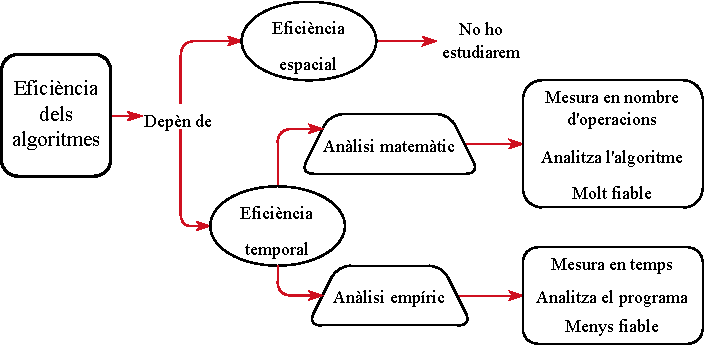
\includegraphics[width=.65\textwidth]{capitols/figures/diagram.drawio (1).pdf}
    \caption[Diagrama de l'eficiència dels algoritmes.]{Diagrama de l'eficiència dels algoritmes. Font: elaboració pròpia.}
    \label{Figura}
\end{figure}


\subsection{Notació de Landau}
Hi ha diverses maneres de mesurar la complexitat algorítmica respecte de l'entrada. Nosaltres utilitzarem la notació de Landau, coneguda també com a O gran o notació asimptòtica.

La notació de Landau proporciona una forma \quotes{aproximada} d'expressar la complexitat d'un algoritme en funció d'$n$ quan $n$ pren valors molt grans. Ens interessa analitzar el pitjor cas possible de l'algoritme perquè ens assegura que independentment del cas, l'algoritme tardarà igual o menys que la complexitat analitzada.

Formalment, la notació de Landau s'utilitza per descriure el comportament asimptòtic de les funcions. Per exemple, si el temps o quantitat de passos necessari per resoldre un problema de mida $n$ ve donat per $f(n) = 3n^2 + 2n -1$. Si eliminem les constants, ja que depenen de l'ordinador on s'executi i, per tant, varien la velocitat però no l'eficiència, i eliminem també els termes de creixement més lent (ja que estem analitzant el $\lim_{n \to \infty} f(n)$). La quantitat d'operacions quedaria determinada per l'expressió $f(n) = n^2$. Per això, vulgarment diem que és un anàlisi aproximat.

En aquesta notació les constants s'eliminen per dos motius: perquè estem analitzant quan $n$ pren valors molt grans, i, per tant, les podem negligir igual que els termes de creixement més lent. I perquè a l'hora d'executar l'algoritme depenent de l'ordinador, compilador, llenguatge de programació, implementació, etc, les constants varien. Per exemple, si la quantitat d'operacions que fa un algoritme ve donada per l'expressió $f(n) = n^2$ i un ordinador A fa 1 operació per segon i un ordinador B fa 4 operacions per segon (un ordinador normal pot fer unes $10^8$ operacions per segon). L'ordinador A tardaria $n^2$ segons, i l'ordinador B tardaria $\frac{n^2}{4}$ segons. Veiem com canviant la velocitat de l'ordinador, però executant el mateix programa i algoritme, obtenim una diferència de velocitat constant. Com que estem analitzant l'eficiència, no la velocitat, podem eliminar les constants.

% En l'exemple anterior del dentista podem veure com les constants (el temps que tarden a atendre cada pacient) poden variar i la quantitat de passos ($n$) que fan els dentistes són els mateixos. Per això, diem que les constants depenen de l'ordinador, i, per tant, es poden eliminar de l'anàlisi d'eficiència.

% No explicaré totes les funcions que es poden expressar en aquesta notació, sinó les més bàsiques i necessàries per a aquest treball. 

\subsubsection*{Complexitat constant $O(1)$}
La primera complexitat és la complexitat constant, i s'expressa de la següent manera: $O(1)$. 

La lletra \quotes{o} majúscula indica la notació que estem utilitzant, per això la notació de Landau també es diu notació O gran. I el que hi ha a l'interior del parèntesi indica el creixement de l'algoritme. En aquest cas hi ha un 1 i no hi ha cap $n$, això vol dir que les operacions no depenen de la mida de l'entrada i sempre, independentment de la seva mida l'algoritme farà la mateixa quantitat d'operacions.

Per exemple, si vols agafar un llibre d'una estanteria d'$n$ llibres i saps que vols el primer. No caldrà que el busquis, podràs agafar el primer fent una única operació. No importa quants llibres hi hagi, sempre faràs una sola operació. Per això, el nombre d'operacions és constant i no depèn d'$n$ (la mida de l'entrada).

Si ara féssim un gràfic d'aquesta complexitat i poséssim a l'eix d'abscisses la mida de l'entrada ($n$), i a l'eix d'ordenades el nombre d'operacions. Obtindríem la figura 1.4.

% -------------------------------------------------------------gràfic complexitat constant
% \begin{wrapfigure}[7]{R}{0.35\textwidth}
\begin{figure}[h]
    % \vspace{-18pt}
    \centering
    \begin{tikzpicture}
        \centering
        \begin{axis}[xmin=0, xmax=100, ymin=0, ymax=8, axis lines = middle, 
        x label style={at={(axis description cs:0.5,-0.1)},anchor=north},
        y label style={at={(axis description cs:-0.1,.5)},rotate=90,anchor=south},
        xlabel={$n$ mida de l'entrada},
        ylabel={nombre d'operacions},
        style={thick}, 
        compat=1.18, width=.35\textwidth]
        \addplot[color=vermellpral, domain=0:100]{1};
        % \addplot[color=verd, domain=0:10]{3};
        \legend{$O(1)$,$O(3)$}
        \end{axis}
    \end{tikzpicture}
    \caption[Gràfic de complexitat constant.]{Gràfic de complexitat constant. Font: elaboració pròpia.}\label{fig:my_label}
\end{figure}

Podem veure com a mesura que l'entrada es va fent cada vegada més gran, el nombre d'operacions es manté constant.

Amb l'anàlisi de complexitats estudiem quant tardarà l'algoritme quan la mida de l'entrada $n$ sigui molt gran. En aquest cas veiem que no creix i que es manté constant. 

Per tant, si hem d'utilitzar un algoritme de complexitat constant per a $n = 1.000.000$, farà la mateixa quantitat d'operacions que per a $n = 10$. I la velocitat d'aquestes operacions dependran completament de factors externs a l'algoritme (ordinador, implementació, etc.).

\subsubsection*{Complexitat lineal $O(n)$}
Aquesta ja depèn de la mida de l'entrada i s'expressa així: $O(n)$. A mesura que incrementa $n$ el temps també incrementa de forma directament proporcional.

Per exemple, si estàs buscant un llibre en una estanteria, hauràs de comprovar cada llibre fins a trobar el que busques. En el pitjor cas possible el llibre estarà situat l'últim a l'estanteria, i hauràs de comprovar-los tots fins a trobar-lo. Si hi ha $n$ llibres, trobar el teu llibre t'haurà costat $n$ operacions com a màxim. Per tant, l'eficiència temporal d'aquest procediment són $n$ operacions, complexitat lineal o $O(n)$.

L'exemple del dentista també té complexitat lineal, ja que fa $n$ visites. Ens és igual si tarden $30 \cdot n$ minuts, $5 \cdot n$ minuts, o qualsevol constant per $n$, ja que creixen de la mateixa manera, linealment. I, perquè en aquesta notació les constants s'eliminen.

En el gràfic 1.5 podem veure que a mesura que incrementa la mida de l'entrada, també incrementa el nombre d'operacions en la mateixa mesura. Per a una mida d'entrada petita el nombre d'operacions incrementa igual de ràpid que per a mides d'entrada més grans. 
% -------------------------------------------------------------gràfic complexitat lineal
% \begin{wrapfigure}[8]{r}{.35\textwidth}
\begin{figure}[H]
% \vspace{-18pt}
\centering
\begin{tikzpicture}
\centering
\begin{axis}[xmin=0, xmax=100, ymin=0, ymax=100, axis lines = middle, 
x label style={at={(axis description cs:0.5,-0.1)},anchor=north},
y label style={at={(axis description cs:-0.1,.5)},rotate=90,anchor=south},
xlabel={$n$ mida de l'entrada},
ylabel={nombre d'operacions},
style={thick}, 
compat=1.18, width=.35\textwidth, 
% legend style={nodes={scale=0.75, transform shape}}, 
legend pos= south east]
\addplot[color=vermellpral, domain=0:100]{x};
\addplot[color=verd, domain=0:100]{5*x};
% \addplot[color=verd, domain=0:10]{3*x};
\legend{$O(n)$, $O(5n)$}
\end{axis}
\end{tikzpicture}
    \caption[Gràfic de complexitat lineal.]{Gràfic de complexitat lineal. Font: elaboració pròpia.}
    \label{fig:my_label}
\end{figure}

% Per tant, un algoritme de complexitat lineal fa tantes operacions com la mida de l'entrada. És a dir, si $n = 10$ farà 10 operacions i si $n = 1.000.000$ farà 1.000.000 d'operacions.

\subsubsection*{Complexitat quadràtica $O(n^2)$}
En aquest tipus d'algoritmes el nombre d'operacions és proporcional al quadrat d'$n$. 

Per exemple, estem al supermercat i tenim una llista de la compra amb $n$ productes. Però abans d'anar a pagar volem comprovar que no ens hàgim deixat res. Així que llegim el primer producte de la llista i el busquem a la nostra cistella, després fem el mateix fins a comprovar els $n$ productes. Cada vegada que busquem el producte a la cistella, estem fent màxim $n$ operacions, és a dir, buscar el producte a la cistella té una complexitat d'$O(n)$. Però estem fent aquest procés tantes vegades com productes apuntats a la llista ($n$). Així que estem fent $n$ operacions $n$ vegades o $n \cdot n = n^2$ operacions. Per tant, l'eficiència temporal d'aquest procediment seria $n^2$ operacions com a màxim.

En el gràfic de la figura 1.6 podem veure clarament com aquesta complexitat és menys eficient que les altres, ja que el nombre d'operacions incrementa molt ràpidament. A diferència de la complexitat anterior, aquesta quan la mida de l'entrada és més petita incrementa més lentament, però a mesura que l'entrada és més gran, el nombre d'operacions incrementa cada vegada més ràpidament. 
% ------------------------------gràfic complexitat lineal
% \begin{wrapfigure}[8]{r}{.35\textwidth}
\begin{figure}[h]
    \centering
    % \vspace{-18pt}
\begin{tikzpicture}
\centering
\begin{axis}[xmin=0, xmax=100, ymin=0, ymax=100, axis lines = middle, 
x label style={at={(axis description cs:0.5,-0.1)},anchor=north},
y label style={at={(axis description cs:-0.1,.5)},rotate=90,anchor=south},
xlabel={$n$ mida de l'entrada},
ylabel={nombre d'operacions},
style={thick}, 
compat=1.18, width=.35\textwidth, 
% legend style={nodes={scale=0.75, transform shape}}, 
legend pos=south east]
\addplot[color=vermellpral, domain=0:10, samples=150]{x^2};
% \addplot[color=verd, domain=0:10]{2*(x^2)};
\legend{$O(n^2)$, $O(2 \cdot n^2)$}
\end{axis}
\end{tikzpicture}
    \caption[Gràfic de complexitat quadràtica.]{Gràfic de complexitat quadràtica. Font: elaboració pròpia.}
    \label{fig:my_label}
\end{figure}

% Per aquesta complexitat podem predir que per a $n = 10$, farà $n^2 = 10^2 = 100$ operacions i per a $n = 1.000.000$ farà $n^2 = 1.000.000^2 = 10^{12}$ operacions. 

Recordem que sempre estem analitzant el pitjor cas possible, així que un algoritme mai farà més operacions de les previstes, però molts cops en farà menys.

\subsubsection*{Complexitat logarítmica $O(\log_2{n})$}
Un algoritme té complexitat logarítmica quan la quantitat d'operacions és proporcional al logaritme d'$n$.

Per exemple: quan busquem una paraula en un diccionari a paper. Per buscar-la primer obrim el diccionari més o menys per la meitat i per ordre alfabètic deduïm si la paraula queda a la dreta o a l'esquerra. Després fem exactament el mateix, però amb una de les meitats i a poc a poc anem fent més petit el rang on podem trobar la paraula. Aquest procés té complexitat logarítmica o $O(\log_2{n})$.

Els logaritmes són la inversa de l'exponencial (una constant elevada a $n$, com $2^n$), i responen a quantes vegades ($v$) la base ($b$) es multiplica a ella mateixa fins a arribar a l'argument ($n$). És a dir $\log_b{n} = v \iff b^v = n$, per exemple: $\log_2{16} = 4 \iff 2^4 = 16$. 

En l'exemple del diccionari per a $n = 16$ partim les pàgines per la meitat, després fem la meitat de la meitat... Així: $16 \rightarrow 8 \rightarrow 4 \rightarrow 2 \rightarrow 1$. Si ens hi fixem, aquesta seqüència és la mateixa que $2^4$ però invertida: $2^4 = 2 \cdot 2^3 = 4 \cdot 2^2 = 8 \cdot 2 = 16$. 

El procediment del diccionari parteix les pàgines exponencialment però de forma inversa, i el logaritme és la inversa de l'exponencial. Per això aquest procediment té complexitat logarítmica.

Una altra forma de resoldre un logaritme és dividir l'argument entre la base $v$ vegades fins a obtenir el quocient d'1. $v$ és el resultat del logaritme. En la figura 1.7 podem veure un exemple amb $\log_2{8} = 3$. És a dir, es necessiten 3 passos per partir 8 dades en 2 meitats fins a obtenir grups d'una dada.
%\begin{wrapfigure}[6]{L}{.4\textwidth}
\begin{figure}[H]
    % \vspace{-18pt}
    \centering
    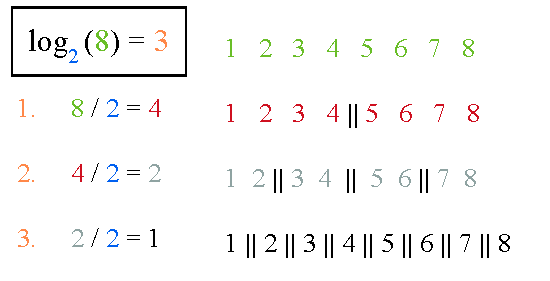
\includegraphics[width=.4\textwidth]{capitols/figures/log (4).pdf}
    % \vspace{-25pt}
    \caption[Relació entre partir nombres i els logaritmes.]{Relació entre partir nombres i els logaritmes. Font: elaboració pròpia.}
    \label{fig:my_label}
\end{figure}
Si el diccionari té $n$ pàgines i $n = 128$, seguint el procediment de l'exemple anterior, haurem de fer $\log_2{n} = \log_2{128} = 7$ passos per arribar a partir-ho en pàgines individuals.  Per això diem que la complexitat d'aquest algoritme és $O(\log_2{n})$.

Si representem aquesta complexitat en el gràfic 1.8, podem veure que quan la mida de l'entrada és més petita, el nombre d'operacions creix més ràpidament, però a mesura que les $n$ són més grans, cada vegada el nombre d'operacions creix més a poc a poc.
% ------------------------------gràfic complexitat log
% \begin{wrapfigure}[8]{R}{.35\textwidth}
\begin{figure}[h]
    \centering
    % \vspace{-18pt}
\begin{tikzpicture}
\centering
\begin{axis}[xmin=0, xmax=100, ymin=0, ymax=100, axis lines = middle, 
x label style={at={(axis description cs:0.5,-0.1)},anchor=north},
y label style={at={(axis description cs:-0.1,.5)},rotate=90,anchor=south},
xlabel={$n$ mida de l'entrada},
ylabel={nombre d'operacions},
style={thick}, 
compat=1.18, width=.35\textwidth]
\addplot[color=vermellpral, domain=-2:100, samples=100]{log2(x)};
\legend{$O(\log_2{n})$}
\end{axis}
\end{tikzpicture}
    \caption[Complexitat logarítmica.]{Complexitat logarítmica. Font: elaboració pròpia.}
    \label{fig:my_label}
\end{figure}



Per tant, per a $n = 10$, farà $\log_2{n} = \lceil\log_2{10}\rceil = 4$ operacions i per a $n = 10^6$ farà $\log_2{n} = \lceil\log_2{10^6}\rceil = 20$ operacions.

\subsubsection*{Totes les complexitats}
Finalment, per comparar les diferents complexitats entre elles, podem fer un gràfic que les representi a totes i una taula amb algunes dades per comparar-les. D'aquesta manera podem veure clarament com la complexitat quadràtica és la pitjor de les que hem explicat, i la complexitat logarítmica és la millor excloent-hi la constant.

Els algoritmes de complexitat constant només es poden utilitzar per a problemes que no depenguin d'$n$, els quals són molt poc comuns i molt senzills, com per exemple operacions matemàtiques. L'algoritme de la figura 1.2, té complexitat constant.
% \begin{wrapfigure}[11]{R}{.45\textwidth}
%     \vspace{-20pt}
%     \centering
% \begin{tikzpicture}
% \begin{axis}[xmin=0, xmax=100, ymin=0, ymax=100, axis lines = middle, 
% x label style={at={(axis description cs:0.5,-0.1)},anchor=north},
% y label style={at={(axis description cs:-0.1,.5)},rotate=90,anchor=south},
% xlabel={$n$ mida de l'entrada},
% ylabel={nombre d'operacions},
% legend pos=south east, 
% style={thick}, 
% compat=1.18, width=.45\textwidth]
% \addplot[color=vermellpral, domain=0:100]{1};
% \addplot[color=taronja, domain=-2:100]{log2(x)};
% \addplot[color=verd, domain=0:100]{x};
% \addplot[color=blau, domain=0:100]{x^2};
% \legend{$O(1)$,$O(log_{2}n)$, $O(n)$, $O(n^2)$}
% \end{axis}
% \end{tikzpicture}
%     \caption{Gràfic amb totes les complexitats. Font: elaboració pròpia.}
%     \label{fig:my_label}
% \end{wrapfigure}

% En aquest gràfic podem veure com la complexitat quadràtica creix molt ràpidament comparat amb les altres, així que els algoritmes amb aquesta complexitat s'haurien d'evitar, sobretot per a $n$ molt grans. Les complexitats constant i logarítmiques són les més ràpides i seria convenient utilitzar algoritmes amb aquestes complexitats per a $n$ molt grans, ja que el nombre d'operacions creix molt a poc a poc en aquest cas. Si per a resoldre un problema podem escollir entre una solució de complexitat quadràtica o logarítmica, doncs ara ja sabem quina solució escollir; la logarítmica.

% \begin{figure}[H]
%     % \vspace{-20pt}
% \centering
% \begin{minipage}{.5\textwidth}
% \begin{tikzpicture}
% \begin{axis}[xmin=0, xmax=100, ymin=0, ymax=100, axis lines = middle, 
% x label styleS={at={(axis description cs:0.5,-0.1)},anchor=north},
% y label style={at={(axis description cs:-0.1,.5)},rotate=90,anchor=south},
% xlabel={$n$ mida de l'entrada},
% ylabel={nombre d'operacions},
% legend pos=north east,
% style={thick}, 
% legend style={nodes={scale=0.75, transform shape}}, 
% compat=1.18, width=.9\textwidth]
% \addplot[color=vermellpral, domain=0:100, samples=100]{1};
% \addplot[color=taronja, domain=-2:100, samples=100]{log2(x)};
% \addplot[color=verd, domain=0:100, samples=100]{x};
% \addplot[color=blau, domain=0:100, samples=100]{x^2};
% \legend{$O(1)$,$O(log_{2}n)$, $O(n)$, $O(n^2)$}
% \end{axis}
% \end{tikzpicture}
%     \caption[Gràfic amb totes les complexitats.]{Gràfic amb totes les complexitats. \\ Font: elaboració pròpia.}
%     \label{fig:my_label}
% \end{minipage}%
% \begin{minipage}{.5\textwidth}
%     \begin{center}
%     \renewcommand{\arraystretch}{1}
%     \begin{tabular}{| l | * {3}{c|}}\hline
%     %  \diagbox[width=.3\textwidth]{\vspace{10pt}\rotatebox{320}{complex}}{$n$}
%     \diagbox[width=.4\textwidth]{complexitat}{$n$}
%      & 10 & 50.000 & $10^{6}$ \\ 
%      \hline
%      \textit{$O(1)$} & 1 & 1 & 1 \\ 
%      \hline
%      \textit{$O(\log_2{n})$} & 4 & 16 & 20 \\
%      \hline
%      \textit{$O(n)$} & 10 & 50.000 & $10^{6}$ \\ 
%     \hline
%     \textit{$O(n^2)$} & 100 & $25 \cdot 10^8$ & $10^{12}$ \\ 
%     \hline
%     \end{tabular}
%     \end{center}
%     \caption[Taula amb exemples del nombre d'operacions per complexitat.]{Taula amb exemples del nombre d'operacions per complexitat. Font: elaboració pròpia.}
%     \label{fig:my_label}
% \end{minipage}
% \end{figure}

\begin{figure}[H]
    \centering
    \begin{tikzpicture}
    \begin{axis}[xmin=0, xmax=200, ymin=0, ymax=200, axis lines = middle, 
    % x label styleS={at={(axis description cs:0.5,-0.1)},anchor=north},
    y label style={at={(axis description cs:-0.1,.5)},rotate=90,anchor=south},
    xlabel={$n$ mida de l'entrada},
    ylabel={nombre d'operacions},
    legend pos= outer north east,
    style={thick}, 
    % legend style={nodes={scale=0.75, transform shape}}, 
    compat=1.18, width=.45\textwidth]
    \addplot[color=vermellpral, domain=0:200, samples=100]{1};
    \addplot[color=taronja, domain=-2:200, samples=200]{log2(x)};
    \addplot[color=verd, domain=0:200, samples=100]{x};
    \addplot[color=blau, domain=0:40, samples=200]{x^2};
\legend{$O(1)$,$O(log_{2}n)$, $O(n)$, $O(n^2)$}
    \end{axis}
    \end{tikzpicture}
    \caption[Gràfic amb totes les complexitats.]{Gràfic amb totes les complexitats. Font: elaboració pròpia.}
    \label{fig:my_label}
\end{figure}
\begin{figure}[H]
    \centering
    \begin{center}
    \renewcommand{\arraystretch}{.8}
    \begin{tabular}{| l | * {5}{c|}}\hline
    %  \diagbox[width=.3\textwidth]{\vspace{10pt}\rotatebox{320}{complex}}{$n$}
    \diagbox[width=.5\textwidth]{Complexitats}{$n$}
     & 10 & 1.000 & 10.000 & 50.000 & $10^{6}$ \\ 
     \hline
     \textit{$O(1)$} & 1 & 1 & 1 & 1 & 1 \\ 
     \hline
     \textit{$O(\log_2{n})$} & 4 & 10 & 14 & 16 & 20 \\
     \hline
     \textit{$O(n)$} & 10 & 1.000 & 10.000 & 50.000 & $10^{6}$ \\ 
    \hline
    \textit{$O(n^2)$} & 100 & $10^6$ & $10^8$ & $25 \cdot 10^8$ & $10^{12}$ \\ 
    \hline
    \end{tabular}
    \end{center}
    \caption[Taula amb exemples del nombre d'operacions per complexitat.]{Taula amb exemples del nombre d'operacions per complexitat. Font: elaboració pròpia.}
    \label{fig:my_label}
\end{figure}%
\vspace{-18pt}
Aquestes quatre complexitats no són totes, també hi ha la complexitat exponencial ($O(2^n)$) i factorial ($O(n!)$) que són molt pitjors que la quadràtica. No les expliquem per què no calen per als objectius d'aquest treball. També hi ha complexitats que es componen de les complexitats bàsiques que hem explicat. Per exemple, si hi ha un algoritme que fa $n$ vegades un procediment logarítmic, la complexitat serà $O(n \cdot \log_2{n})$. 

\chapter{Anàlisi matemàtic}
% The contact list in your phone is sorted, which means you can easily access your desired contact from your phone since the data is arranged in that manner for you. In other words, “it is sorted”.

% While shopping on flip kart or amazon, you sort items based on your choice, that is, price low to high or high to low.

% used in programming TV to sort channels based on audience viewing time!
% \section{Nomenclatura}
% Una llista és una seqüència de qualsevol valor. Per exemple: $llistaA: 4, 5, 6, 7$. La \textit{llistaA} és una llista ordenada ascendentment de nombres naturals consecutius amb 4 elements.

% Per accedir a cada element de la llista utilitzarem la seva posició o índex començant per 0. Ho podem expressar d'aquesta manera per exemple, $llistaA[0] = 4$. A l'índex 0 de la \textit{llistaA} hi ha l'element 4.
% \begin{figure}[h]
%     \begin{center}
%     \renewcommand{\arraystretch}{1.5}
%     \begin{tabular}{|c | c | c | c | c |} 
%      \hline
%      \textit{LlistaA} & 4 & 5 & 6 & 7 \\ 
%      \hline
%      Índex & 0 & 1 & 2 & 3 \\
%      \hline
%     \end{tabular}
%     \end{center}
%     \caption{Llistes i posicions.}
%     \label{fig:my_label}
% \end{figure}    

% En aquesta llista hi ha $n = 4$ elements, així que el primer element és $LlistaA[0]$, i l'últim element és $LlistaA[n-1]$.

% Per tant, per obtenir tots els elements de la llista, haurem de mirar tots els índexs entre 0 i $n-1$ ambdós inclosos.

Hi ha dos problemes bàsics i essencials que han de poder resoldre tots els dispositius. Aquests són: la cerca i l'ordenació. L'ordenació consisteix a ordenar un conjunt de dades. I la cerca consisteix a trobar la posició d'una dada en un conjunt.

Com tots els problemes hi ha moltes formes de solucionar-los, per això explicaré dos algoritmes per cada problema i els analitzarem per determinar el més eficient. En el següent capítol implementarem els algoritmes.

% Aquests dos problemes els trobem en moltes situacions, per exemple: les paraules d'un diccionari estan ordenades per facilitar la cerca d'una paraula. Quan ordenem el menjar segons la data de caducitat. O quan ordenem els valors de la borsa en funció dels beneficis en un període de temps determinat. O quan busques una paraula en un document, quan cerques un producte a la pàgina d'una botiga... 

Aquests dos problemes els podem trobar en algoritmes que resolen tasques més complexes i que en el seu funcionament requereixen resoldre aquestes tasques més simples. I per optimitzar aquests algoritmes més complexos, podem començar optimitzant una part de l'algoritme com pot ser la resolució d'una cerca o ordenació.
\section{Cerca}
Aquest problema consisteix a trobar la posició d'una dada en un conjunt. En aquest treball, per simplicitat, utilitzarem un conjunt d'$n$ nombres enters. Per tant, aquest problema té dues entrades: el nombre que cerquem, que anomenarem $k$, i una llista o seqüència d'$n$ nombres. 

Com que la sortida del problema és la posició o índex de $k$ a la llista, hem de definir quin índex té cada nombre. En programació normalment es comença a indexar des de zero, així que el primer element té índex 0, el segon té índex 1 així fins a $n-1$. Per exemple:
\begin{figure}[h]
    \begin{center}
    \renewcommand{\arraystretch}{1.5}
    \begin{tabular}{|c | c | c | c | c |} 
     \hline
     \textit{Llista} & 48 & 5 & 12 & 83 \\ 
     \hline
     Índex & 0 & 1 & 2 & 3 \\
     \hline
    \end{tabular}
    \end{center}
    \caption{Llistes i índex.}
    \label{fig:my_label}
\end{figure} 

Veiem com la llista té $n = 4$ elements, així que l'últim element té l'índex d'$n-1 = 4-1 = 3$. 

Per exemple, si les entrades d'un problema de cerca són la llista de la figura 2.1, i $k = 5$. Hem de trobar la posició de $k = 5$ en la $Llista = \lbrace 48, 5, 12, 83 \rbrace$. De manera que la sortida seria 1. Ja que la posició de $k = 5$ en la llista té índex = 1. També ho podriem expressar com $Llista_1 = 5$, ja que a l'índex 1 de la llista hi ha l'element 5.

\subsection{Cerca lineal}
L'algoritme de cerca lineal consisteix a mirar cada element un per un i comprovar si coincideixen amb el que estem buscant ($k$). Aquest algoritme acaba quan trobem l'element o hem comprovat tota la llista.

% Com diu el nom de l'algoritme, té complexitat lineal. De fet, l'exemple de complexitat lineal del capítol anterior és un algoritme de cerca lineal. 
Per exemple, si tenim una $Llista = \lbrace 6, 2, 1, 8, 4 \rbrace$ i $k = 8$. L'algoritme faria el següent:

Anomenem $i$ l'índex del nombre que estem comprovant ($i$ incrementa a cada pas). Així, quan es compleix $Llista_i = k$, la sortida serà igual a $i$.

\begin{enumerate}
    \item Comprova el primer element ($Llista_0 = 6$), com que aquest no és igual a $k = 8$, passa al següent, $i = i + 1$.
    \item $Llista_1 = 2$, com que $2 \neq k$, passa al següent.
    \item Després comprova $i = 2$ com que $Llista_2 \neq k$ comprovem el següent.
    \item Finalment $Llista_3 = k$, la sortida és $i = 3$ i acaba l'algoritme.
\end{enumerate}

Ho podem representar gràficament amb la figura 2.2.
% \begin{wrapfigure}[7]{R}{.45\textwidth}
\begin{figure}[h]
    % \vspace{-18pt}
    \centering
    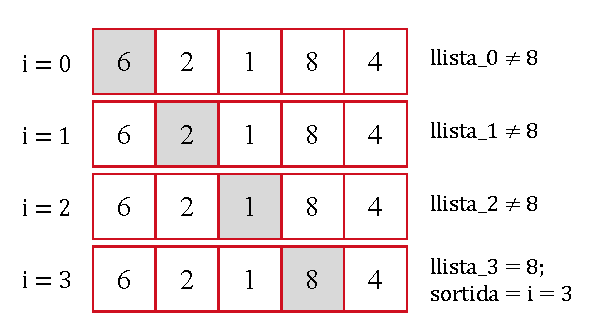
\includegraphics[width=.45\textwidth]{capitols/figures/linearsearch (2).pdf}
    \caption[Cerca lineal.]{Cerca lineal. Font: elaboració pròpia.}
    \label{fig:my_label}
\end{figure}

Pot passar que l'element no estigui a la llista, en aquest cas comprovaríem els $n$ elements i quan acabés la llista, acabaria l'algoritme.

El pitjor cas possible de la cerca lineal és que l'element se situï en l'última posició o que no hi sigui a la llista. En ambdós casos hauríem de comprovar els $n$ elements, per això aquest algoritme té complexitat lineal o $O(n)$. Les operacions per comparar si l'element coincideix, són constants (no depenen d'$n$), per això les podem eliminar de l'analisi de complexitats.

La implementació de la cerca lineal la podeu trobar a \textcolor{red}{l'annex 2.}

\subsection{Cerca dicotòmica}
L'algoritme de la cerca dicotòmica resol el mateix problema que la cerca lineal, però amb el requisit que la llista ha d'estar ordenada. Aquest algoritme és el mateix que el de l'exemple del diccionari de la complexitat logarítmica. 

Aquest algoritme consisteix a acotar el rang on podem trobar l'element fins que només en queda un i coincideix amb el que busquem. Per acotar el rang partim la llista per la meitat, i com que està ordenada, podem saber en quina meitat es troba $k$, de manera que a cada pas podem descartar la meitat dels elements que ens quedaven.

% \begin{wrapfigure}[7]{R}{.52\textwidth}
%     \vspace{-18pt}
%     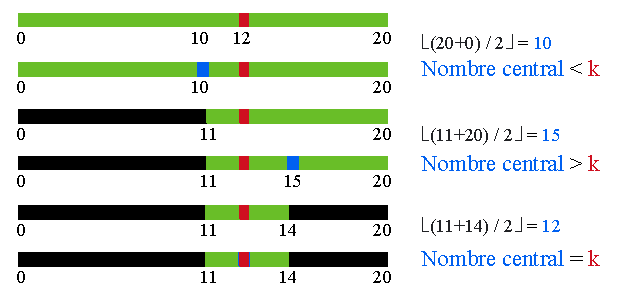
\includegraphics[width=.52\textwidth]{capitols/figures/binarysearch (2).pdf}
%     \caption[Exemple 1. Cerca dicotòmica.]{Exemple 1. Cerca dicotòmica. Font: elaboració pròpia.}
%     \label{fig:my_label}
% \end{wrapfigure}

% En la figura 2.3 hi ha un exemple en que $n = 21$ i $k = 12$. Inicialment, $k$ (franja vermella) pot estar en el rang sencer de la llista (franja verda), ja que encara no hem fet cap operació. El primer que fa l'algoritme és trobar el nombre central (franja blava) del rang 0 - 20 que és 10, i com que $k > 10$ podem suposar que $k$ està a la dreta del nombre central. Així que podem acotar el rang, $k$ es troba entre el nombre central exclòs i el nombre més gran, és a dir, 11 - 20. Ara repetim el mateix, però amb el nombre central d'entre 11 i 20 que és 15. Com que $k < 15$ sabem que $k$ està a l'esquerra del nombre central, entre 11 i 14, ja que excloem el 15. Repetim el mateix en el rang 11 - 14, el centre és 12. Com que $k = 12$, ja hem trobat el nombre i acaba l'algoritme.

% Tot aquest procés es realitza amb els índexs dels nombres de la llista, d'aquesta manera, no cal que els nombres siguin consecutius, només cal que estiguin ordenats. 

% En l'exemple de la figura 2.3, per simplicitat i perquè s'entengui millor l'algoritme, els nombres són consecutius de 0 a 20, de manera que els índexs coincideixen amb els valors. Normalment, la llista no és de nombres consecutius de manera que no pots suposar la posició del valor que busques. L'exemple de la figura 2.4 és més acurat.

Per exemple, si tenim la $Llista = \lbrace 2, 4, 7, 12, 24, 38, 51, 56, 62, 65, 71, 83, 89, 98, 99 \rbrace$, $n = 15$ i $k = 62$. L'algoritme faria el següent:

% En la figura 2.4 $k$ pot estar en el rang sencer, 0 - 14, i la dada del centre és a l'índex $\frac{0+14}{2} = 7$. $Llista_7 = 56$, $56 < k$, així que sabem que $k$ estarà entre l'índex 8 i el 14. La dada central d'aquest rang és $\frac{8+14}{2} = 11$, $Llista_{11} = 83$, $83 > k$. Per tant, sabem que $k$ està en un índex més petit o igual a 10 i més gran o igual a 8. Així que el centre és $\frac{8+10}{2} = 9$, $Llista_9 = 65, 65 > k$ així que sabem que $k$ està entre 8 i 8. Com que $Llista_8 = 62 = k$, acabem l'algoritme i la sortida és 8.

\begin{enumerate}
\item $k$ es troba en el rang 0 - 14 ambdós inclosos, per tant,  calculem en quin índex queda la dada central, així, $\frac{0+14}{2} = 7$. Com que $k$ és més gran que la dada de l'índex 7, podem descartar totes les posicions més petites a l'índex 7 inclòs. És a dir, com que $Llista_7 = 56 < k$  podem assegurar que $k$ es troba en el rang 8 - 14 ambdós inclosos.
\item Repetim el pas 1 però en el rang 8 - 14 ambdós inclosos. La dada central es troba a l'índex $\frac{8+14}{2} = 11$. Com que $LLista_{11} = 83 > k$, $k$ es troba a l'esquerra de l'índex 11, en el rang 8 - 10 ambdós inclosos. 
\item Trobem la dada central de 8 - 10, $\frac{8+10}{2} = 9$, $Llista_9 = 65 > k$ . Per tant, $k$ es troba en el rang 8 - 8.
\item La dada central de 8 - 8 es troba en $\frac{8+8}{2} = 8$, $Llista_8 = 62 = k$. Per tant, acaba l'algoritme i la sortida és 8. 
\end{enumerate}

Ho podríem representar gràficament en la figura 2.3. Els elements en verd representen els que no han estat descartats, els que estan en blau representen les dades centrals, i en vermell representen $k$.

\begin{figure}[h]
    \centering
    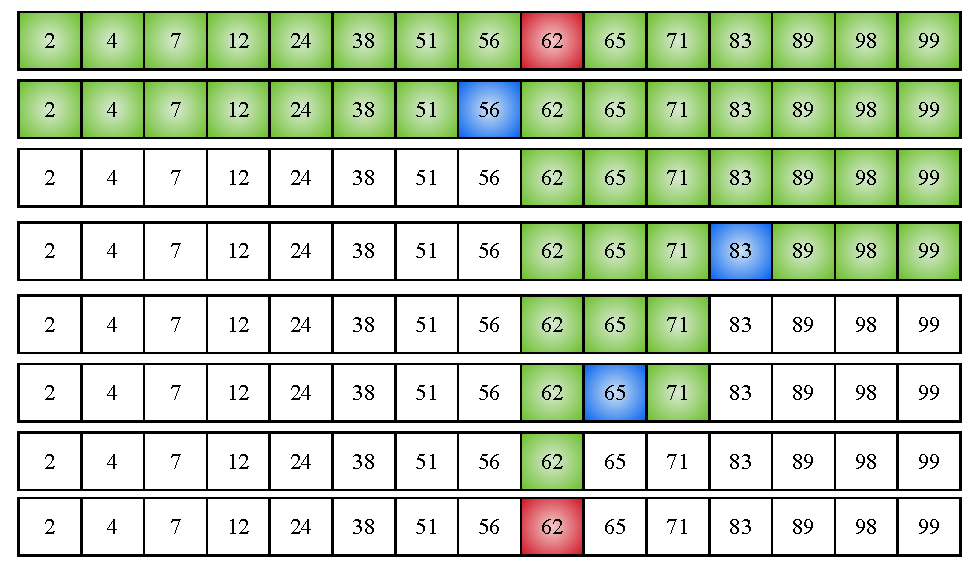
\includegraphics[width=.65\textwidth]{capitols/figures/binary2.pdf}
    \caption[Exemple 2. Cerca dicotòmica.]{Exemple 2. Cerca dicotòmica. Font: elaboració pròpia.}
    \label{fig:my_label}
\end{figure}
El pitjor cas possible és que $k$ no es trobi a la llista, ja que hauríem d'arribar a partir les dades d'una en una per assegurar-nos que no ho estigui. Això també ha passat en l'exemple de la figura 2.3, encara que $k$ estigués a la llista. En canvi, si haguéssim escollit $k = 82$, haguésim acabat l'algoritme partint les dades una sola vegada.

Com hem explicat al punt 1.2.2 a la complexitat logarítmica, aquest algoritme té complexitat logarítmica, ja que $\lceil\log_2{n}\rceil$ és la quantitat necessària de passos per partir les dades de la manera com ho fa la cerca dicotòmica. En la figura 1.7 es pot veure com es parteixen les dades igual que en aquest algoritme, i la relació que té amb els logaritmes.

Com hem vist, a cada partició de les dades s'ha de buscar la dada central i resoldre una inequació. Com que aquestes operacions són constants (no depenen d'$n$), les podem eliminar de l'analisi de complexitats, i ens queda que aquest algoritme té complexitat $O(\log_2{n})$.

La implementació de la cerca dicotòmica la podeu trobar a \textcolor{red}{l'annex 3.}

\section{Ordenació}
Els problemes d'ordenació consisteixen a ordenar un conjunt de dades. En aquest treball ordenarem ascendentment nombres enters.

L'entrada d'aquest problema és una llista d'$n$ elements. I la sortida consisteix en els $n$ elements ordenats ascendentment.

Hi ha molts algoritmes diferents per resoldre aquest problema, i tots tenen avantatges i inconvenients. En aquest treball ens centrem només en l'eficiència temporal, però hi ha molts altres factors que també afecten l'eficiència de l'algoritme i depèn de la situació cal tenir-ho en conte. N'hi ha que són molt ràpids, però ocupen molta memòria (ordenació per barreja), en canvi, n'hi ha que són més lents, però ocupen menys memòria (ordenació de bombolla), n'hi ha que són més ràpids si hi ha moltes dades repetides, n'hi ha que són específics per a estructures de dades determinades (llistes, heaps, grafs, maps...).

\subsection{Ordenació de bombolla}
Aquest algoritme consisteix a intercanviar dos elements adjacents si no estan en ordre.

Per exemple, si tenim una $Llista = \lbrace7, 2, 5, 3, 11\rbrace$ i $n = 5$, l'algoritme faria el següent:

\begin{enumerate}
    \item Comprovem el primer i segon element (7 i 2), com que $7 > 2$ els intercanviem. I ens queda $Llista = \lbrace2, 7, 5, 3, 11\rbrace$.
    \item Comprovem el segon i tercer element. Com que $7 > 5$, els intercanviem. I queda $Llista = \lbrace2, 5, 7, 3, 11\rbrace$.
    \item Comprovem el tercer i quart element. Com que $7 > 3$, els intercanviem. I queda $Llista = \lbrace2, 5, 3, 7, 11\rbrace$.
    \item Comprovem el quart i cinquè element. Com que $7 < 11$, no els intercanviem. I la llista queda igual $Llista = \lbrace2, 5, 3, 7, 11\rbrace$.
    \item Ara ja hem acabat la llista, i hem de repetir el mateix procediment $n$ vegades en total. \\ Comprovem el primer i segon element. Com que $2 < 5$, queden igual. I queda $Llista = \lbrace2, 5, 3, 7, 11\rbrace$.
    \item Comprovem el segon i tercer element. Com que $5 > 3$, els intercanviem. I queda $Llista = \lbrace2, 3, 5, 7, 11\rbrace$.
    \item Ara la llista ja està ordenada, però els ordinadors no ho poden saber si no ho comproven. I no ho comproven perquè això faria l'algoritme molt lent, ja que cada comprovació té complexitat lineal. Això fa que en un ordinador aquest algoritme segueixi funcionant fins a repetir aquest procés un total d'$n$ vegades, encara que no es canviarà d'ordre cap dada. De manera que no hi ha un pitjor cas possible, ja que en tots els casos es farà la mateixa quantitat d'operacions.
\end{enumerate}

Aquest algoritme itera tota la llista d'$n$ elements $n$ vegades, per tant, fa $n \cdot n = n^2$ operacions. Per això aquest algoritme té complexitat quadràtica o $O(n^2)$. 

Igual que en la cerca, l'algoritme resol inequacions que tenen complexitat constant, i, per tant, no cal tenir-les en compte, ja que depenen de l'ordinador.

\subsection{Ordenació per barreja} %merge
El funcionament d'aquest algoritme el podríem partir en dues parts: en la primera part parteix les dades igual que en la cerca dicotòmica (figura 2.4), i en la segona part les ajunta fins que queden en una sola llista ordenades (figura 2.5). Així:

\begin{figure}[H]
    \centering
    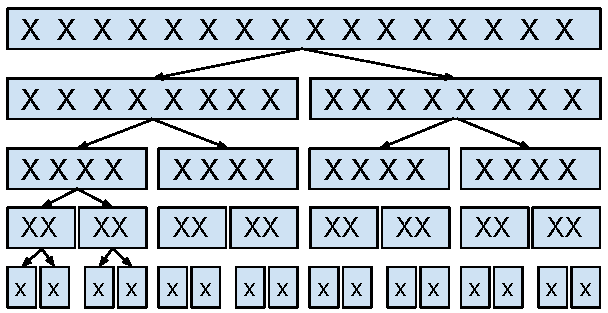
\includegraphics[width=.6\textwidth]{capitols/figures/merge.pdf}
    \caption[Divisió de les dades.]{Divisió de les dades. Font: elaboració pròpia.}
    \label{fig:my_label}
\end{figure}
\vspace{-.8cm}
En la figura 2.4 podem veure com cada llista es parteix per la meitat fins a quedar dades individuals. Igual que en la cerca dicotòmica, i, per tant, també té complexitat logarítmica.
% \vspace{-.5cm}
\begin{figure}[H]
    \centering
    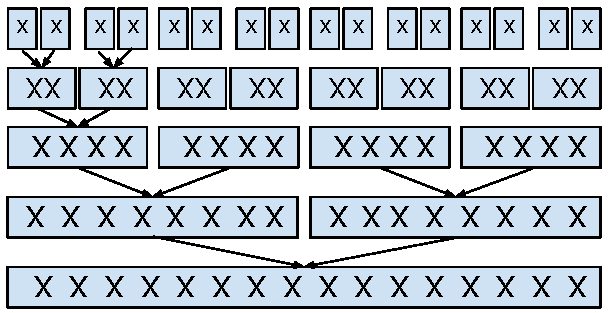
\includegraphics[width=.6\textwidth]{capitols/figures/merge2.pdf}
    \caption[Ajuntar les dades.]{Ajuntar les dades. Font: elaboració pròpia.}
    \label{fig:my_label}
\end{figure}
\vspace{-.5cm}
\begin{wrapfigure}[10]{R}{.35\textwidth}
\vspace{-18pt}
    \centering
    \includegraphics[width=.35\textwidth]{capitols/figures/Còpia de merge2.pdf}
    \caption[Exemple d'ajuntar les dades.]{Exemple d'ajuntar les dades. Font: elaboració pròpia.}
    \label{fig:my_label}
\end{wrapfigure}
Ajuntar les dades és molt simple. Com que comencem amb dades individuals sempre són grups de dades ordenades, per això les podem ordenar tan ràpidament. Primer mirem la dada més petita dels dos grups que volem ajuntar, és a dir, la primera. Després posem la més petita de les dues a la següent llista i avancem una posició a la llista d'on hem tret la dada. Ho podem representar gràficament amb la figura 2.6.

Aquest procediment es repeteix cada vegada que s'ajunten dues llistes.

Podem posar un exemple d'aquest algoritme per a $n = 8$ i $Llista = \lbrace5, 2, 4, 7, 1, 3, 2, 6\rbrace$ en la figura 2.7.

\begin{figure}[H]
    \centering
    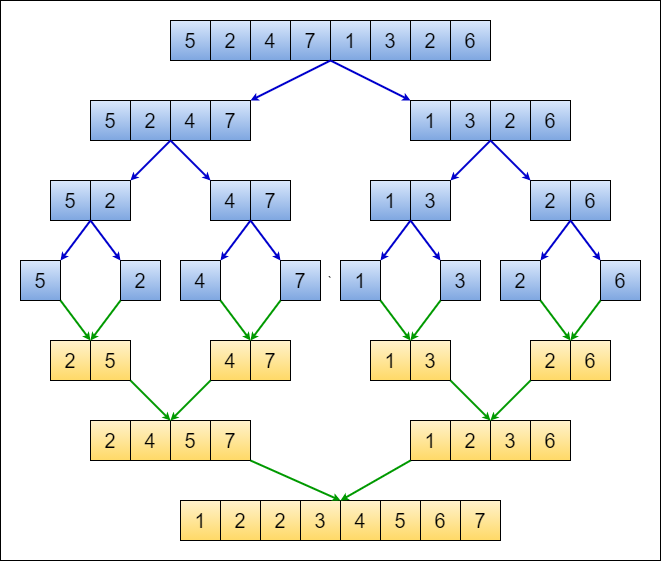
\includegraphics[width=.5\textwidth]{capitols/figures/merge5.png}
    \caption[Exemple d'ordenació per barreja.]{Exemple d'ordenació per barreja. Font: https://levelup.gitconnected.com/visualizing-designing-and-analyzing-the-merge-sort-algorithm-cf17e3f0371f.}
    \label{fig:my_label}
\end{figure}

\vspace{-18pt}
En la primera part de l'algoritme (part blava) només es parteixen les dades, i en la segona part (part groga) s'ajunten com hem vist a la figura 2.6 fins a obtenir una sola llista.

Analitzarem la complexitat d'aquest algoritme separant la part blava de la groga, i després sumarem els dos resultats. La part blava com ja hem vist anteriorment té complexitat logarítmica. I la part groga té complexitat $O(n \cdot log_2{n})$.

En la figura 2.6 hem ajuntat dues llistes de 3 elements per obtenir una llista d'$n = 6$, i hem fet $n$ operacions, ja que hem recorregut cada llista una vegada. De manera que el procediment d'ajuntar dues llistes té complexitat lineal.

En la part groga de la figura 2.7 hi ha les mateixes particions que en la part blava però invertides. És a dir, hi ha $\log_2{n}$ passos a la part groga, i a cada pas ajuntem els $n$ elements de forma lineal. Els ajuntem en llistes diferents de mides diferents, però la suma d'aquestes subllistes tenen mida $n$. Així que en total fem un procediment lineal $\log_2{n}$ vegades, o expressat d'una altra manera $O(n \cdot \log_2{n})$.

Si ho ajuntem tot ens queda una complexitat de $O(\log_2{n} + n \cdot \log_2{n}) \equiv O(n \cdot \log_2{n})$, ja que en l'últim pas podem eliminar el primer $\log_2{n}$ ja que és un terme de creixement més lent.



\chapter{Comprovació empírica}
L'objectiu d'aquest capítol és entendre millor els algoritmes que hem explicat amb una visualització del seu funcionament i implementar-los en un llenguatge de programació per demostrar de forma pràctica les complexitats que hem analitzat al capítol anterior.

\section{Visualització dels algoritmes}
El programa de la figura 3.1 és una visualització dels algoritmes que hem explicat. Aquest representa gràficament les dades en rectangles proporcionals, i executa un algoritme. Els gràfics s'actualitzen a cada pas de l'algoritme, i d'aquesta manera podem veure perfectament el funcionament de cada un. 

També mesura quant tarda cada un i guarda les dades en un document .csv. Aquestes dades no ens serveixen per comprovar la complexitat dels algoritmes, ja que els gràfics rellenteixen molt el funcionament de cada algoritme. Ja que estan implementats per ser visualitzats no per ser molt eficients.

Aquest programa l'he fet en python, ja que és un llenguatge de programació que té bones llibreries gràfiques.

El programa està en aquest enllaç: https://github.com/JordinaGR/TDR-visualitzacio-algoritmes o escanejant el codi de la figura 3.1.

\begin{figure}[H]
    \centering
    
\includegraphics[width=.15\textwidth]{capitols/figures/qrviz.png}
    \caption[Codi QR que porta a una pàgina web amb el codi del programa.]{Codi QR que porta a una pàgina web amb el codi del programa. Font: elaboració pròpia.}
    \label{fig:my_label}
\end{figure}

falta el vídeo

\section{Anàlisi empíric dels algoritmes proposats}
En aquest apartat implementarem els algoritmes que hem explicat, els executarem per a mides d'entrada diferents i farem un gràfic amb els resultats. Més tard compararem el gràfic que obtinguem amb el gràfic de la complexitat analitzada matemàticament en el capítol 2.

Aquest cop he implementat els algoritmes en c++, ja que és un llenguatge de programació més ràpid que python. 

El programa en c++ executa l'algoritme i escriu les dades en un document .csv. Després he fet un altre programa en python per calcular la mitjana del temps que tarden els algoritmes amb la mateixa mida d'entrada utilitzant la llibreria pandas, i generar un gràfic amb la llibreria matplotlib.

A l'hora d'executar el programa per recollir les mostres per fer els gràfics, m'he assegurat que l'ordinador no estigués fent altres tasques alhora. De manera que el rendiment de l'ordinador sempre sigui el mateix i minimitzar al màxim els factors externs a l'execució del programa.

El programa està en aquest enllaç: \url{https://github.com/JordinaGR/TDR-complexitat-algs} o escanejant el codi de la figura 3.2.

\begin{figure}[H]
    \centering
    
\includegraphics[width=.15\textwidth]{capitols/figures/qralgs_complex.png}
    \caption[Codi QR que porta a una pàgina web amb el codi del programa]{Codi QR que porta a una pàgina web amb el codi del programa. Font: elaboració pròpia.}
    \label{fig:my_label}
\end{figure}

\subsubsection{Anàlisi empíric de la cerca lineal}
He executat aquest algoritme un total de 68.000 vegades. Per evitar errors he executat 10 vegades cada mida d'entrada diferent i he calculat la mitjana. Les mides d'entrada les he augmentat en 10 unitats en el rang de 10 a 60.000 i de 60.050 a 100.000 les he augmentat en 50 unitats.

Després he representat les dades en un gràfic de dispersió, i he obtingut el següent resultat:
\begin{figure}[H]
    \centering
    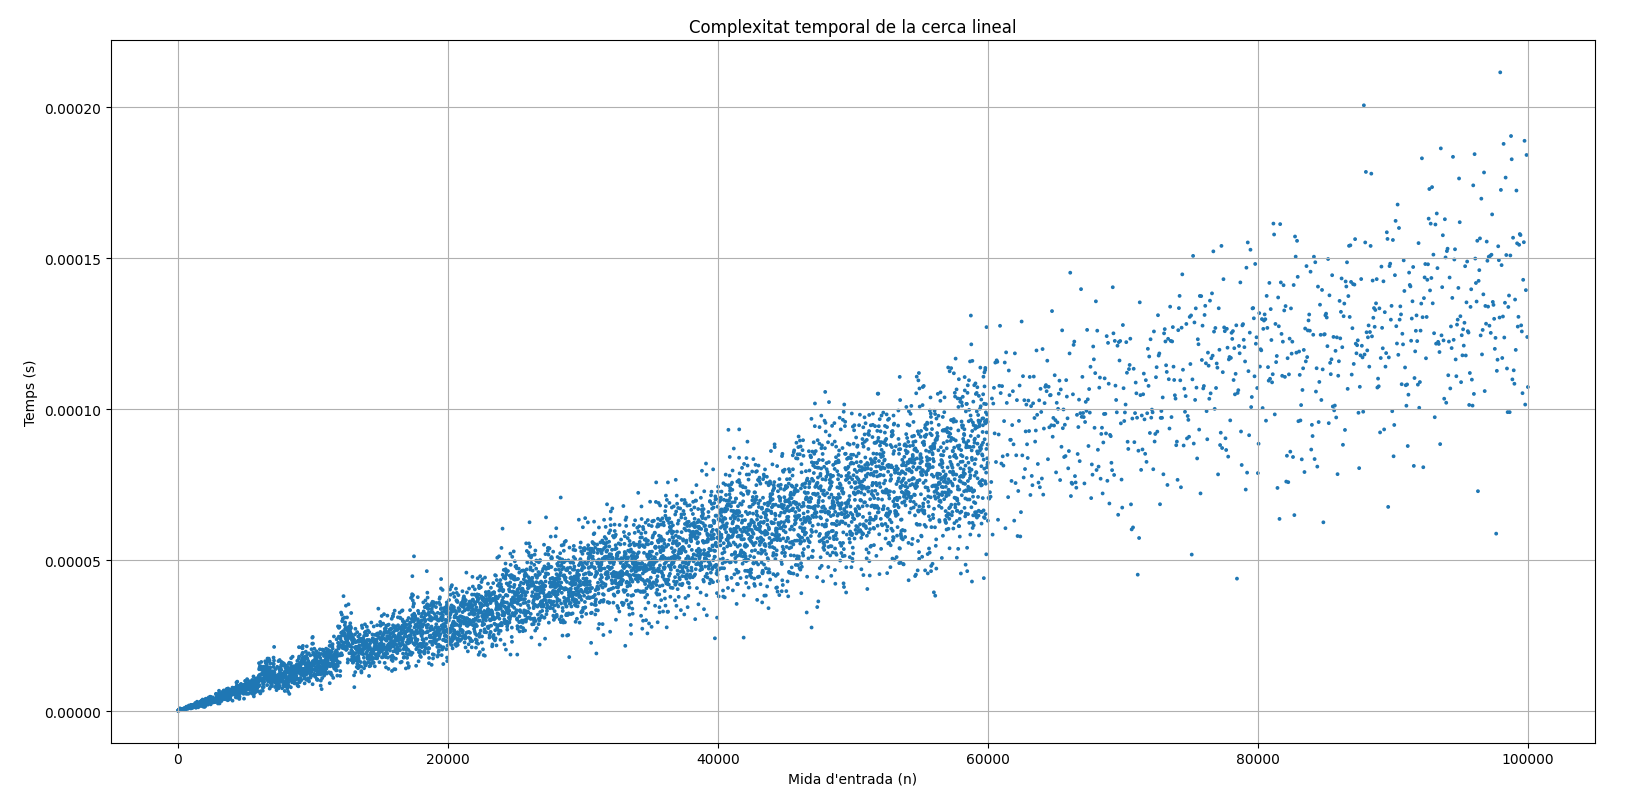
\includegraphics[width=1\textwidth]{capitols/figures/linearplot3.png}
    \caption[Gràfic de dispersió de la cerca lineal.]{Gràfic de dispersió de la cerca lineal. Font: elaboració pròpia.}
    \label{fig:my_label}
\end{figure}

Podem veure en el gràfic de la figura 3.2 una certa relació entre les dues variables. No podem trobar una fórmula que determini el comportament d'aquest programa, ja que hi ha molts factors que afecten els resultats (ordinador, compilador, la dada a cercar...). En canvi, el que podem fer és buscar una correlació entre les dues variables.

En el gràfic 3.2 hi ha una correlació lineal, ja que el gràfic s'aproxima a una recta. Aquesta recta la podem trobar programant amb la llibreria scipy. I obtenim el gràfic 3.3:
\begin{figure}[H]
    \centering
    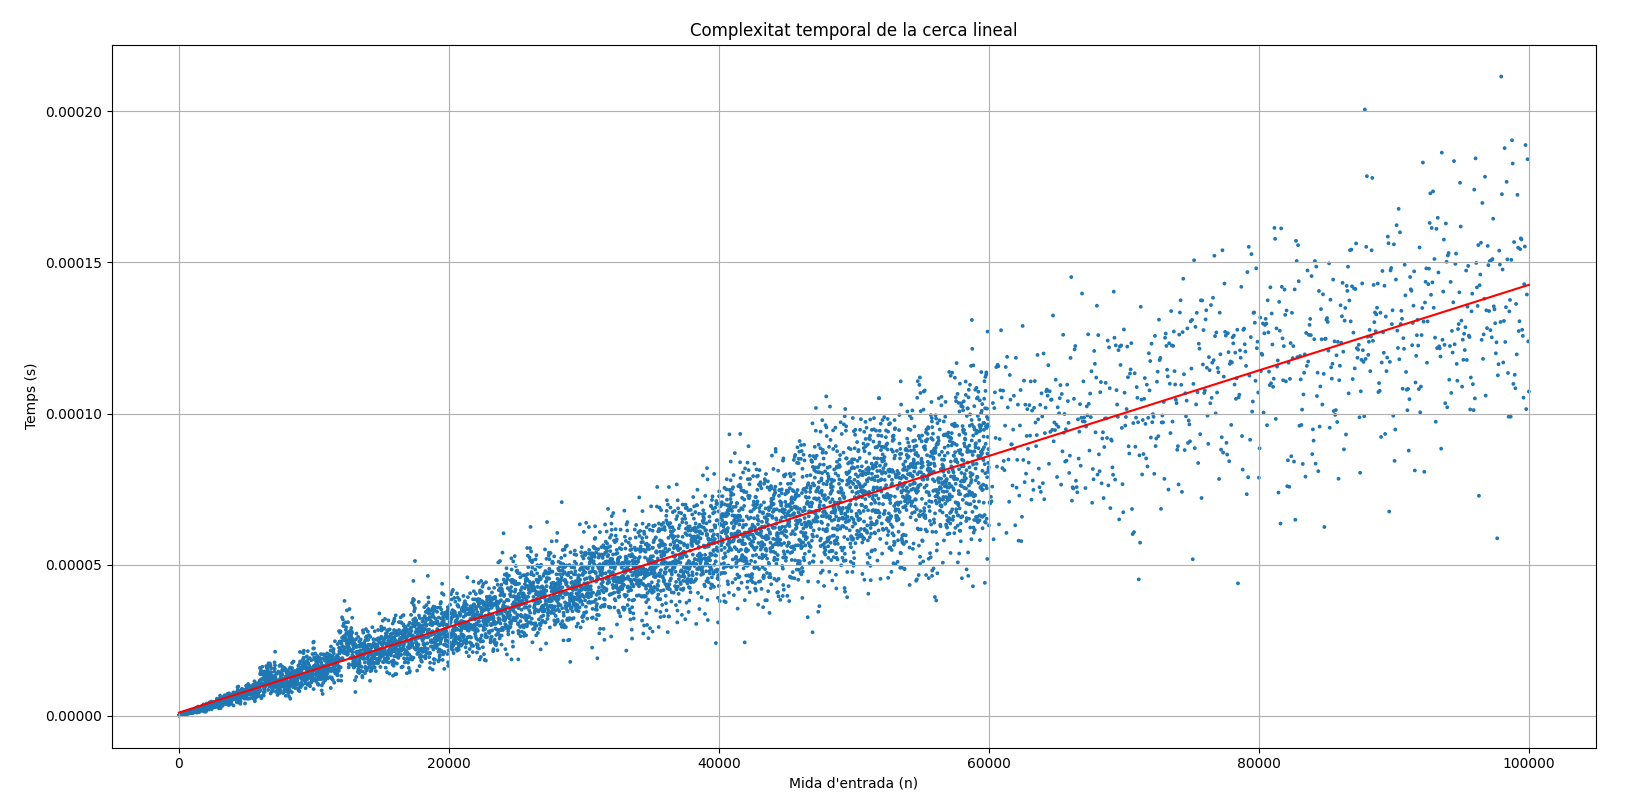
\includegraphics[width=1\textwidth]{capitols/figures/linearplot2.png}
    \caption[Gràfic de dispersió de la cerca lineal amb la recta de correlació lineal.]{Gràfic de dispersió de la cerca lineal amb la recta de correlació lineal. Font: elaboració pròpia.}
    \label{fig:my_label}
\end{figure}

La recta en vermell és la recta que més s'acosta a tots els punts del gràfic.

Si comparem els resultats teòrics que concloïen que la cerca lineal té complexitat $O(n)$ i tornem a fer un gràfic per comparar els resultats.
\begin{figure}[H]
% \vspace{-18pt}
\centering
\begin{tikzpicture}
\centering
\begin{axis}[xmin=0, xmax=200, ymin=0, ymax=400, axis lines = middle, 
x label style={at={(axis description cs:0.5,-0.1)},anchor=north},
y label style={at={(axis description cs:-0.1,.5)},rotate=90,anchor=south},
xlabel={$n$ mida de l'entrada},
ylabel={nombre d'operacions},
style={thick}, 
compat=1.18, width=.4\textwidth, 
% legend style={nodes={scale=0.75, transform shape}}, 
legend pos= south east]
\addplot[color=vermellpral, domain=0:200]{x};
% \addplot[color=verd, domain=0:10]{3*x};
\legend{$O(n)$}
\end{axis}
\end{tikzpicture}
    \caption[Gràfic de complexitat lineal.]{Gràfic de complexitat lineal. Font: elaboració pròpia.}
    \label{fig:my_label}
\end{figure}

Podem veure clarament com els dos gràfics són lineals i, per tant, analitzant la cerca lineal de forma matemàtica i empírica hem arribat al mateix resultat.

En el gràfic 3.4 podem veure que com més creix la mida de l'entrada, les mostres s'allunyen més de la recta. Això és perquè com més gran és la mida de l'entrada, la dada que busquem $k$ pot prendre més valors diferents. És a dir, el programa pot fer entre 1 i $n$ operacions, i com més gran és $n$ més gran és el rang, i per això tenim resultats molt diferents. 

Per comprovar que això és cert, podem executar les mateixes 68.000 mostres per al mateix algoritme, però sent $k$ l'últim element de la llista en tots els casos. D'aquesta manera hem obtingut els següents gràfics:
\begin{figure}[H]
    \centering
    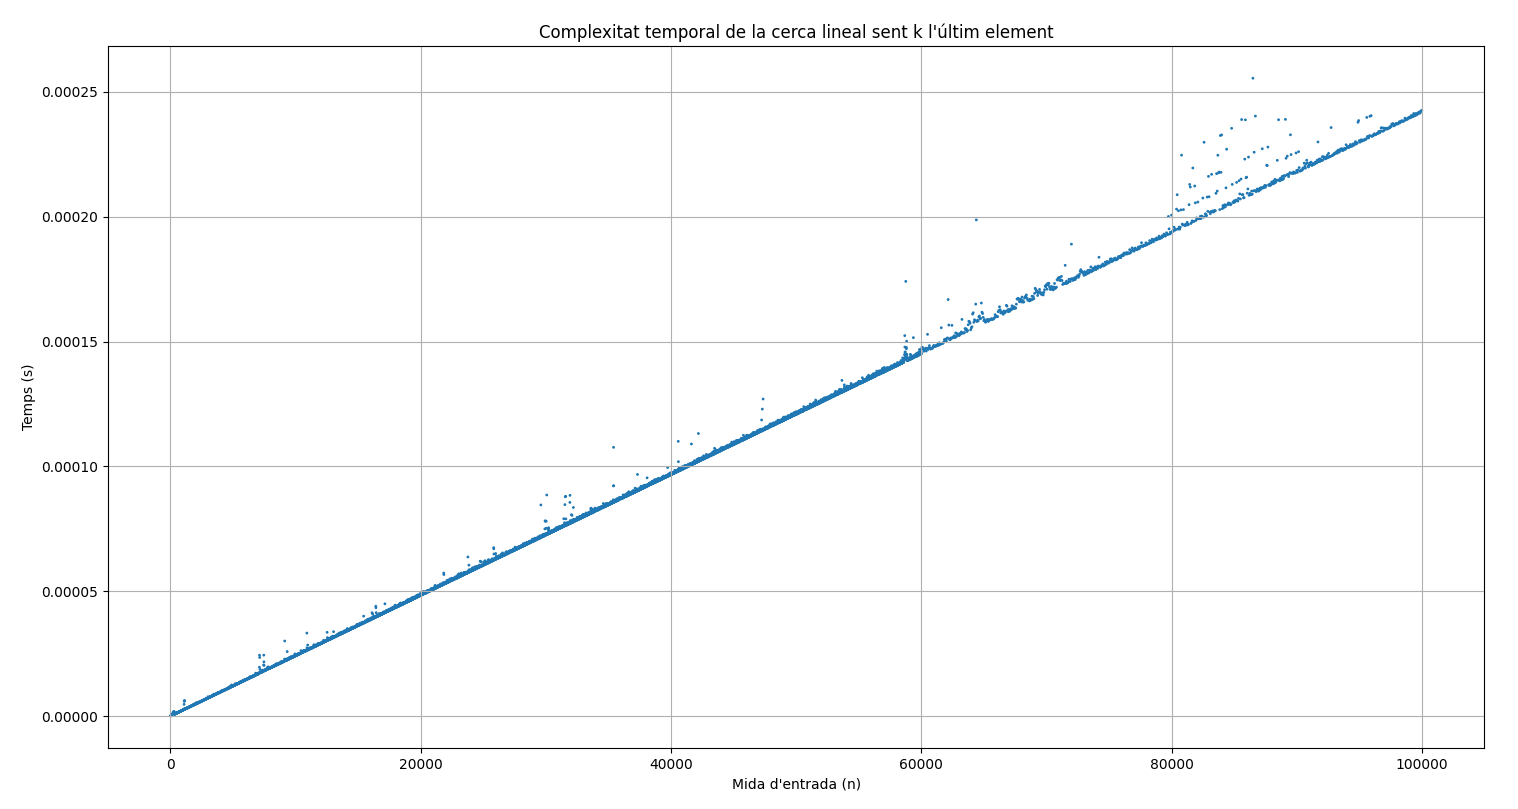
\includegraphics[width=1\textwidth]{capitols/figures/llinerascatter.png}
    \caption[Gràfic de dispersió de la cerca lineal sent $k$ l'últim element.]{Gràfic de dispersió de la cerca lineal sent $k$ l'últim element. Font: elaboració pròpia.}
    \label{fig:my_label}
\end{figure}
\begin{figure}[H]
    \centering
    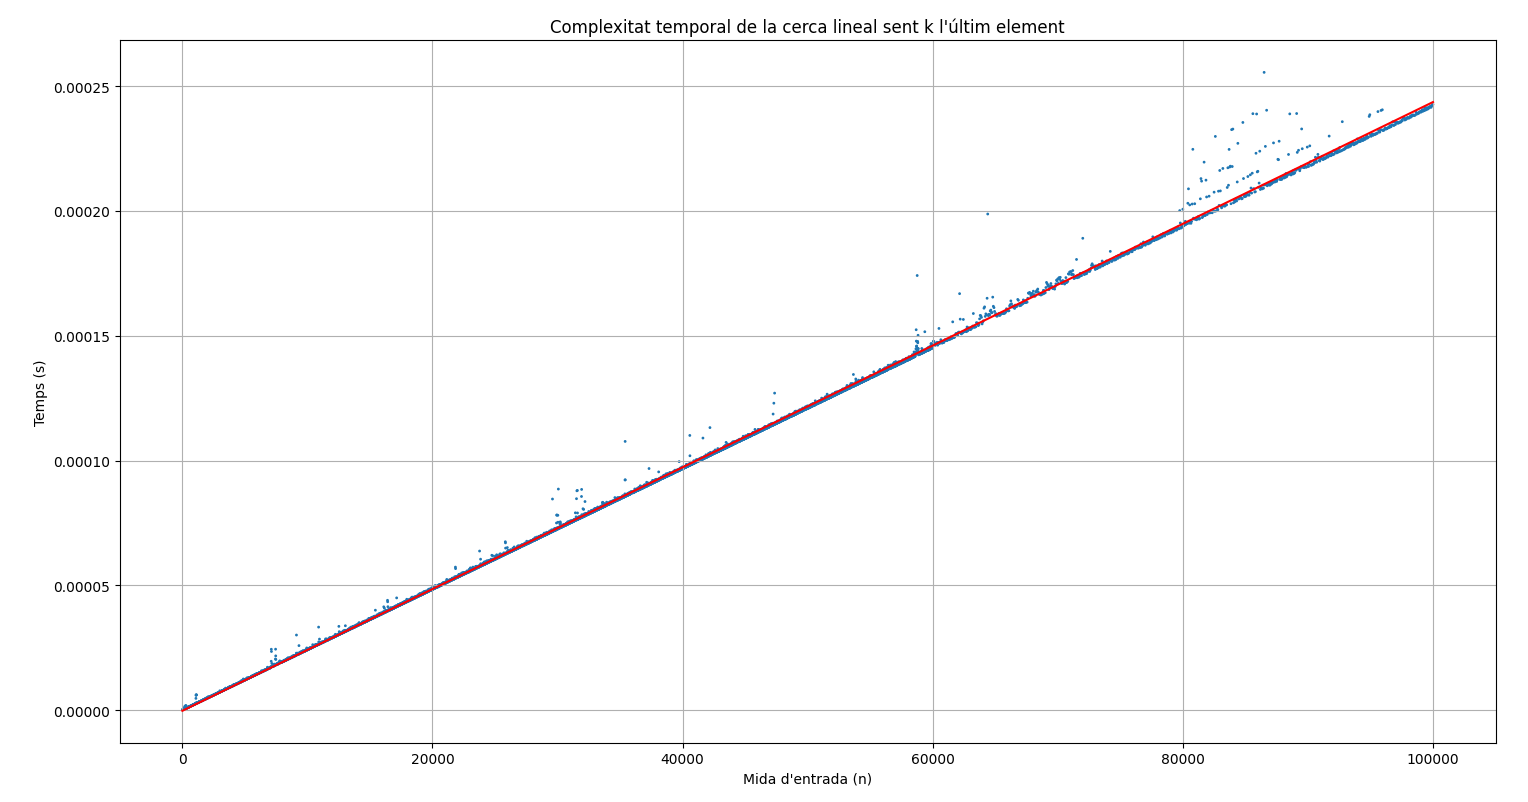
\includegraphics[width=1\textwidth]{capitols/figures/llinearscatterline.png}
    \caption[Gràfic de dispersió de la cerca lineal amb la recta de regressió lineal i sent $k$ l'últim element.]{Gràfic de dispersió de la cerca lineal amb la recta de regressió lineal i sent $k$ l'últim element. Font: elaboració pròpia.}
    \label{fig:my_label}
\end{figure}

En aquests gràfics podem veure de forma més clara que són lineals. A més, la recta de regressió lineal encaixa perfectament amb les mostres que hem obtingut. A més, totes les mostres que s'allunyen de la recta, queden sempre per sobre i mai per sota. Això demostra que quan hi ha hagut algun error, el programa ha tardat més en executar-se i això es pot deure a factors com l'ordinador, sistema operatiu... 

Si comparem els pendents de les rectes, la recta de regressió lineal del gràfic de la figura 3.4 té un pendent de $1.39748 \cdot 10^9$ i la recta del gràfic de la figura 3.7 té un pendent de $2.43812 \cdot 10^9$. És correcte que el pendent de la recta que hem obtingut en l'algoritme en què hem executat el pitjor cas possible sigui superior que en el cas en què $k$ era aleatori. 

Així que podríem tornar a executar l'algoritme en un tercer cas en què $k$ es trobi sempre al centre. D'aquesta manera hauríem d'obtenir una recta més semblant a la de la figura 3.4, però amb els resultats molt més propers a la recta, com en la figura 3.7.

Hem obtingut els següents gràfics:
\begin{figure}[H]
    \centering
    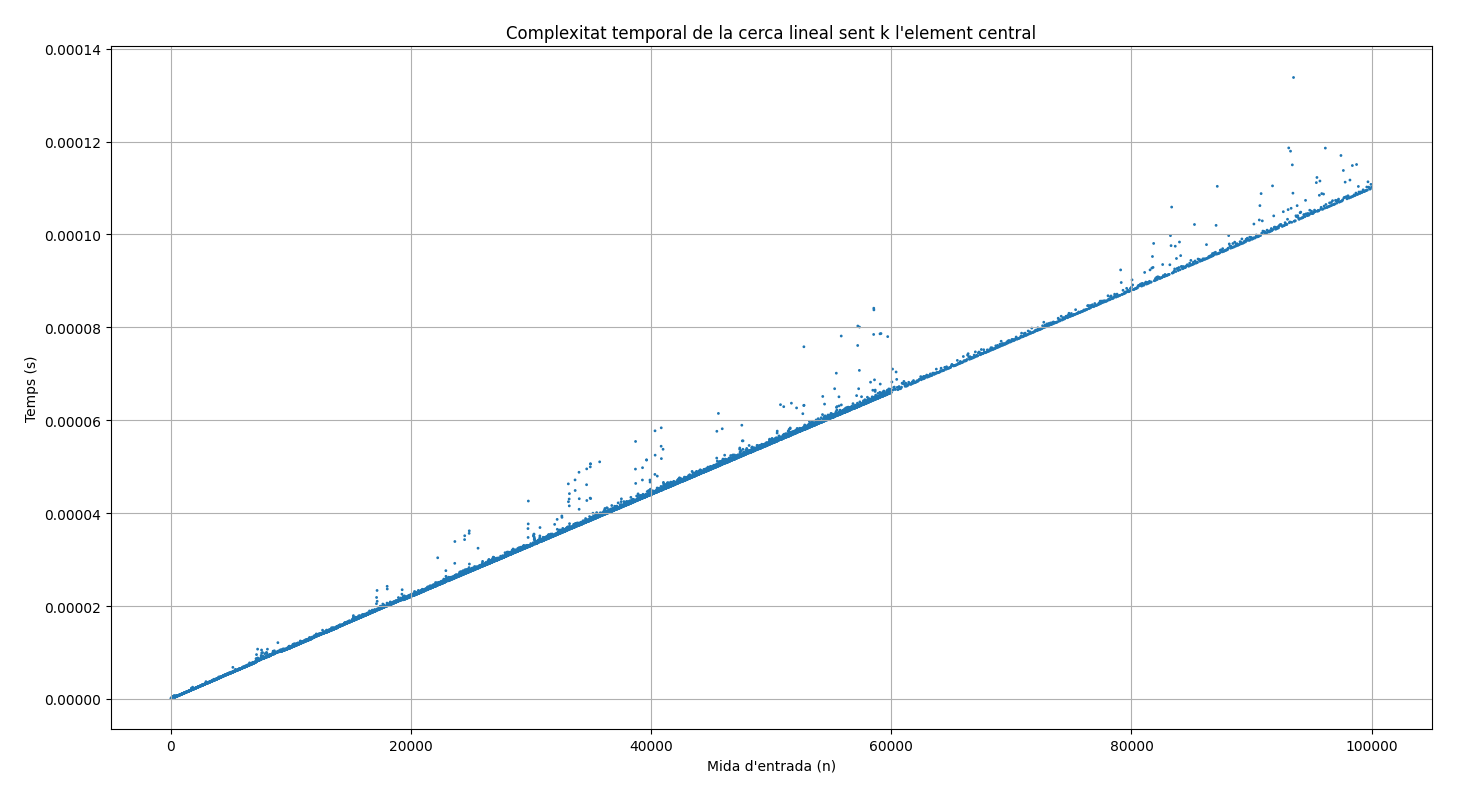
\includegraphics[width=1\textwidth]{capitols/figures/linearmidscatter.png}
    \caption[Gràfic de dispersió de la cerca lineal sent $k$ l'element central.]{Gràfic de dispersió de la cerca lineal sent $k$ l'element central. Font: elaboració pròpia.}
    \label{fig:my_label}
\end{figure}
\begin{figure}[H]
    \centering
    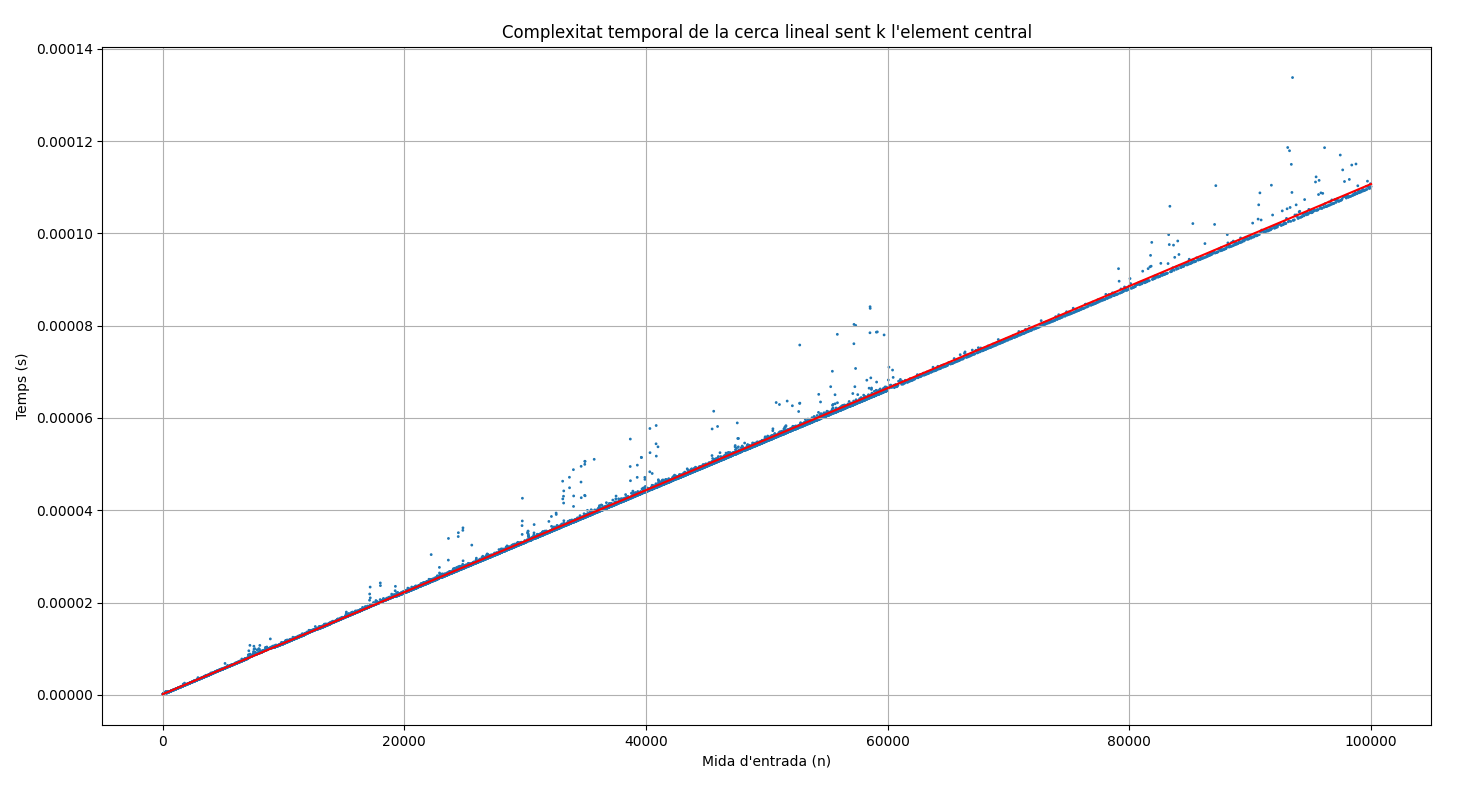
\includegraphics[width=1\textwidth]{capitols/figures/linearmidscatterline.png}
    \caption[Gràfic de dispersió de la cerca lineal amb la recta de regressió lineal i sent $k$ l'element central.]{Gràfic de dispersió de la cerca lineal amb la recta de regressió lineal i sent $k$ l'element central. Font: elaboració pròpia.}
    \label{fig:my_label}
\end{figure}

El pendent de la recta del gràfic de la figura 3.9 és d'$1.10601 \cdot 10^9$ el qual s'aproxima al de la recta del gràfic 3.4 i les mostres són molt més properes a la recta, com havíem predit.

\subsubsection{Anàlisi empíric de la cerca dicotòmica}
Ja que aquest algoritme és més eficient que el de la cerca lineal, he pogut recopilar més mostres. He executat l'algoritme 401.610 vegades. L'he executat 10 vegades per cada mida d'entrada entre 10 i 200.000 en intervals de 10 unitats. Com que entre l'interval d'entre 1 i 10.000 hi havia molt d'error, he recopilat més mostres.

Finalment he obtingut els següents gràfics:
\begin{figure}[H]
    \centering
    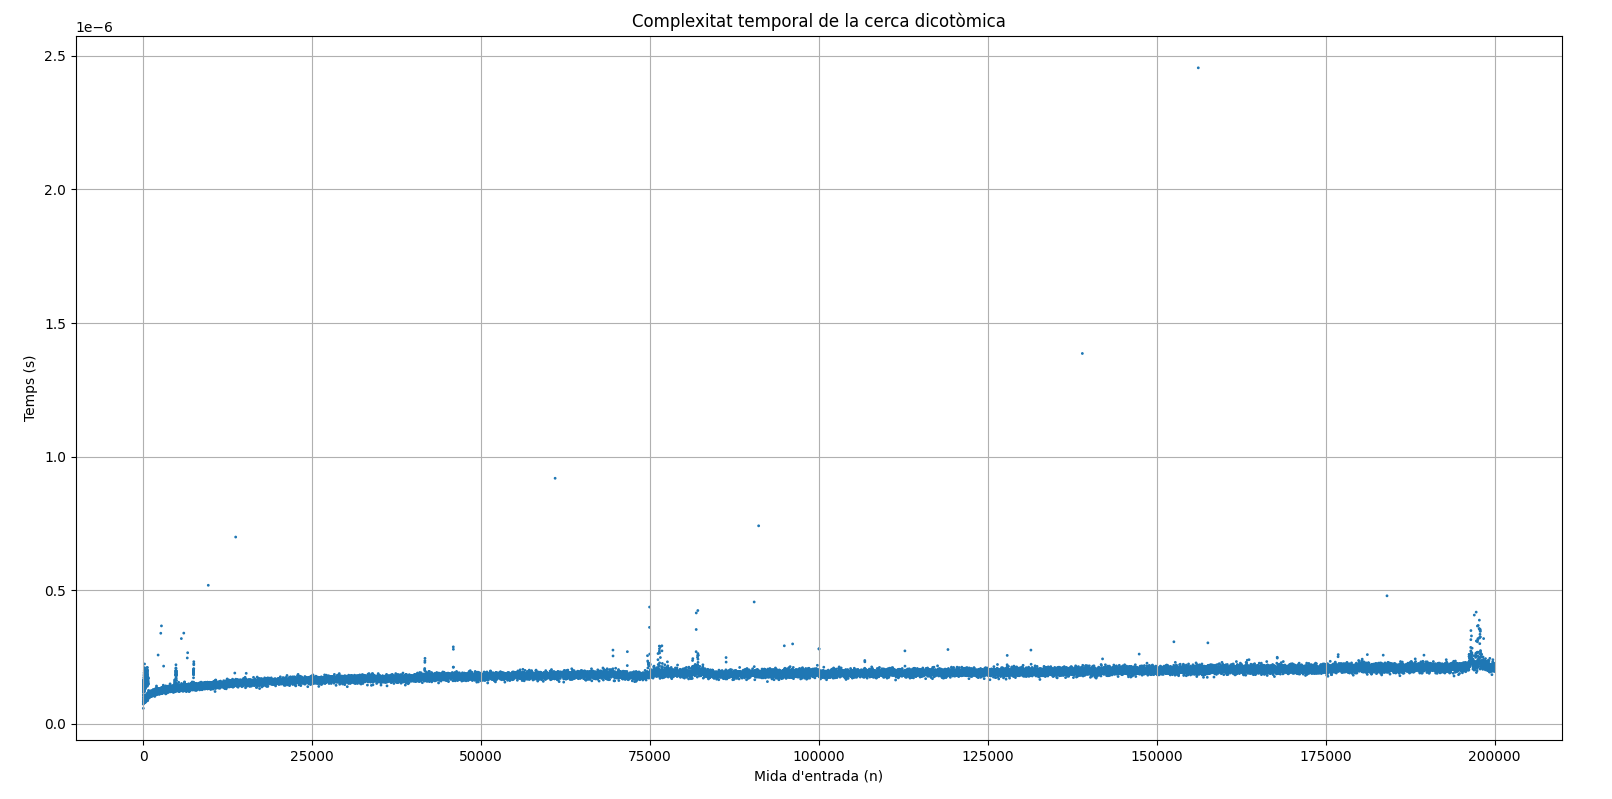
\includegraphics[width=1\textwidth]{capitols/figures/dicotomicagrafic.png}
    \caption[Gràfic de dispersió de la cerca dicotòmica.]{Gràfic de dispersió de la cerca dicotòmica. Font: elaboració pròpia.}
    \label{fig:my_label}
\end{figure}
\begin{figure}[H]
    \centering
    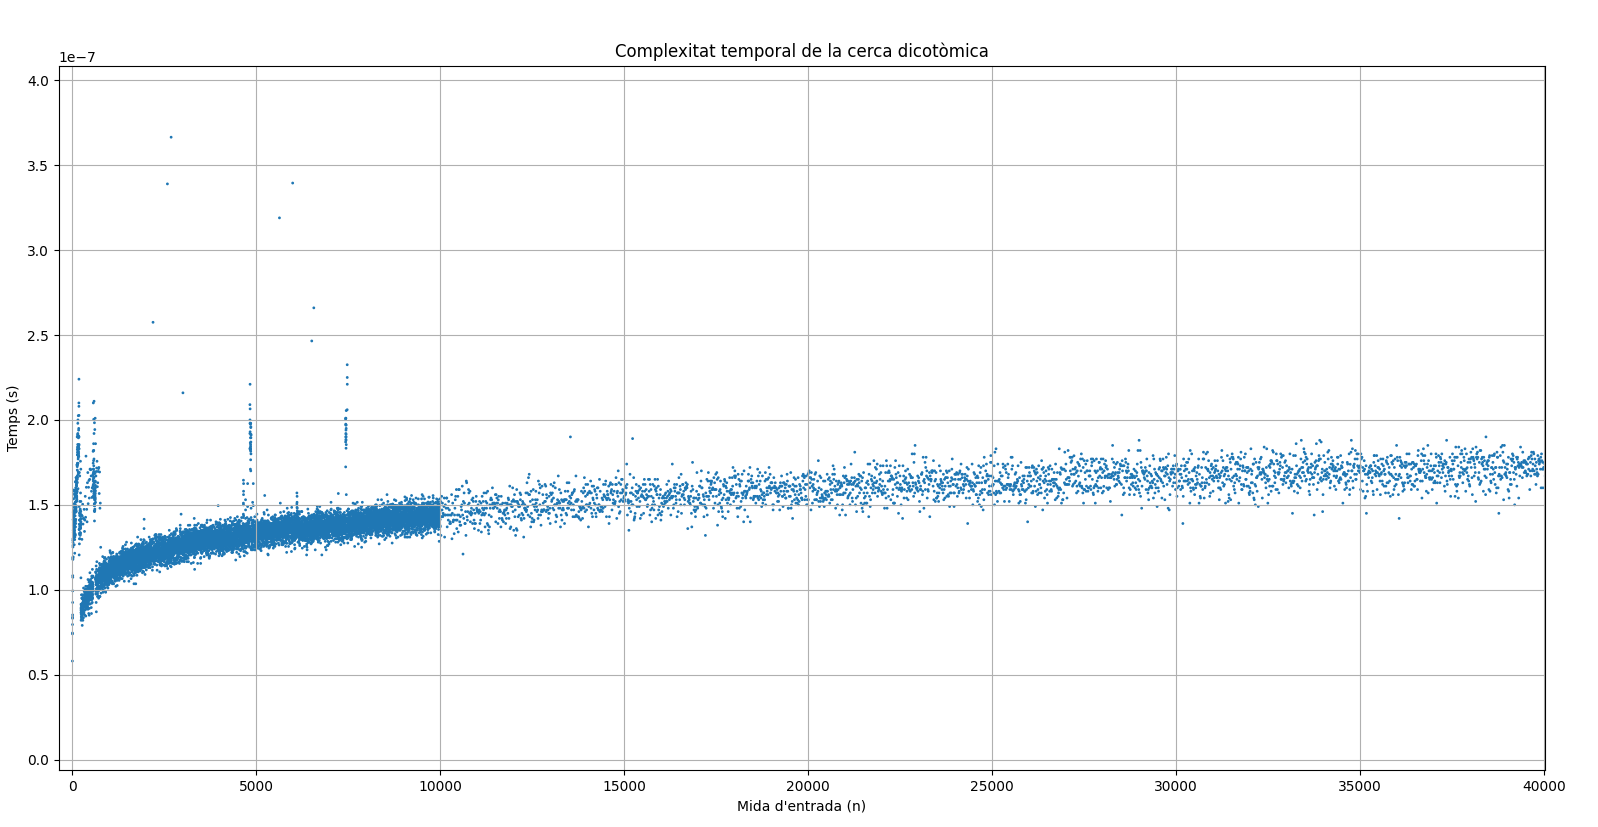
\includegraphics[width=1\textwidth]{capitols/figures/dicotomicaampliat.png}
    \caption[Gràfic de dispersió de la cerca dicotòmica entre l'interval 1 - 40.000.]{Gràfic de dispersió de la cerca dicotòmica entre l'interval 1 - 40.000. Font: elaboració pròpia.}
    \label{fig:my_label}
\end{figure}
\begin{figure}[H]
    \centering
    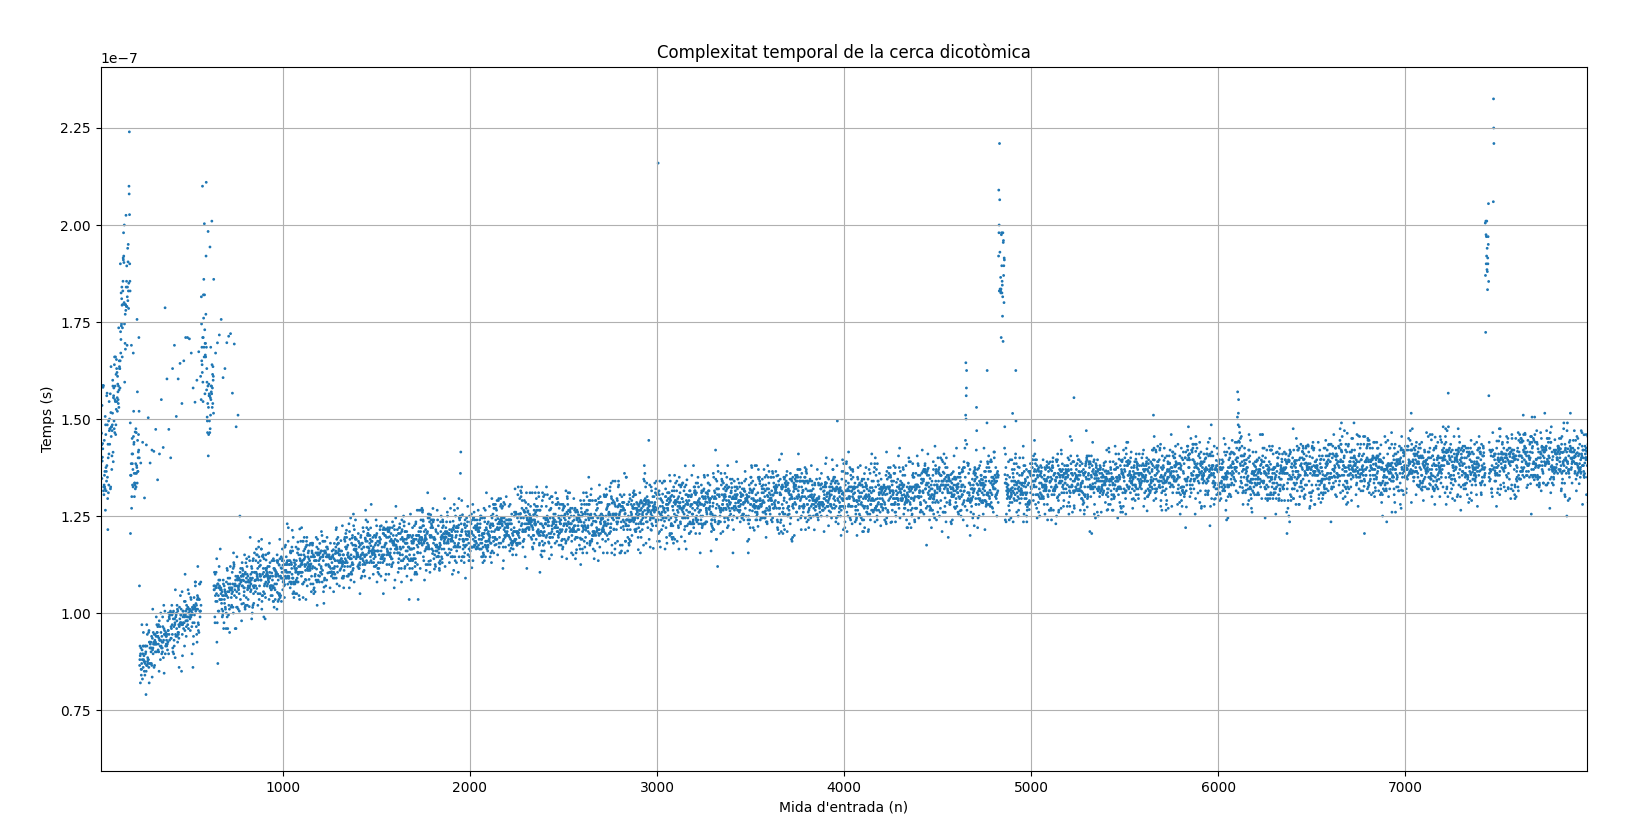
\includegraphics[width=1\textwidth]{capitols/figures/zoomin.png}
    \caption[Gràfic de dispersió de la cerca dicotòmica entre l'interval 1 - 8.000.]{Gràfic de dispersió de la cerca dicotòmica entre l'interval 1 - 8.000. Font: elaboració pròpia.}
    \label{fig:my_label}
\end{figure}

Podem veure que aquests gràfics tenen la mateixa forma que la funció logarítmica.

\begin{figure}[H]
    \centering
    % \vspace{-18pt}
\begin{tikzpicture}
\centering
\begin{axis}[xmin=0, xmax=300, ymin=0, ymax=40, axis lines = middle, 
x label style={at={(axis description cs:0.5,-0.1)},anchor=north},
y label style={at={(axis description cs:-0.1,.5)},rotate=90,anchor=south},
xlabel={$n$ mida de l'entrada},
ylabel={nombre d'operacions},
style={thick}, 
compat=1.18, width=.4\textwidth]
\addplot[color=vermellpral, domain=-2:300, samples=150]{log2(x)};
\legend{$O(\log_2{n})$}
\end{axis}
\end{tikzpicture}
    \caption[Complexitat logarítmica.]{Complexitat logarítmica. Font: elaboració pròpia.}
    \label{fig:my_label}
\end{figure}

Si comparem els gràfics de les figures 3.8 i 3.9 podem veure que els dos tenen la mateixa forma. Per tant, hem demostrat de forma pràctica i teòrica que la cerca dicotòmica té complexitat logarítmica.

També podem veure que en aquests gràfics les mostres no s'allunyen tant com en la cerca lineal, així que podem arribar a la conclusió que la posició de $k$ no afecta gaire els resultats, tampoc quan la mida de l'entrada és molt gran.

\subsubsection{Anàlisi empíric de l'ordenació de bombolla}
Aquest algoritme l'he executat 15.837 vegades. L'he executat 10 vegades per cada mida d'entrada entre 1 i 8.000 en intervals de deu unitats, i 10 vegades entre 8.000 i 10.000 en intervals de 50 unitats.

He obtingut els següents gràfics:
\begin{figure}[H]
    \centering
    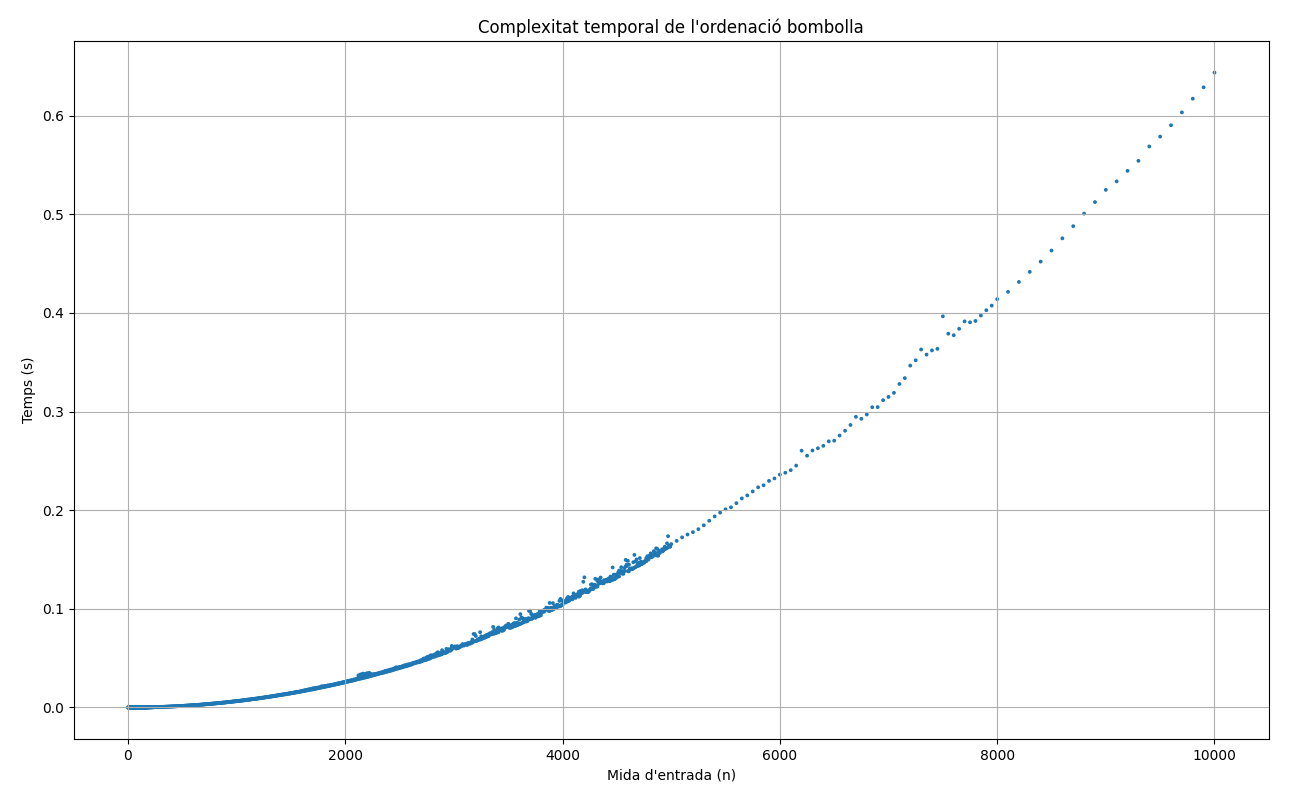
\includegraphics[width=1\textwidth]{capitols/figures/bombollascater2.png}
    \caption[Gràfic de dispersió de l'ordenació bombolla.]{Gràfic de dispersió de l'ordenació bombolla. Font: elaboració pròpia.}
    \label{fig:my_label}
\end{figure}
\begin{figure}[H]
    \centering
    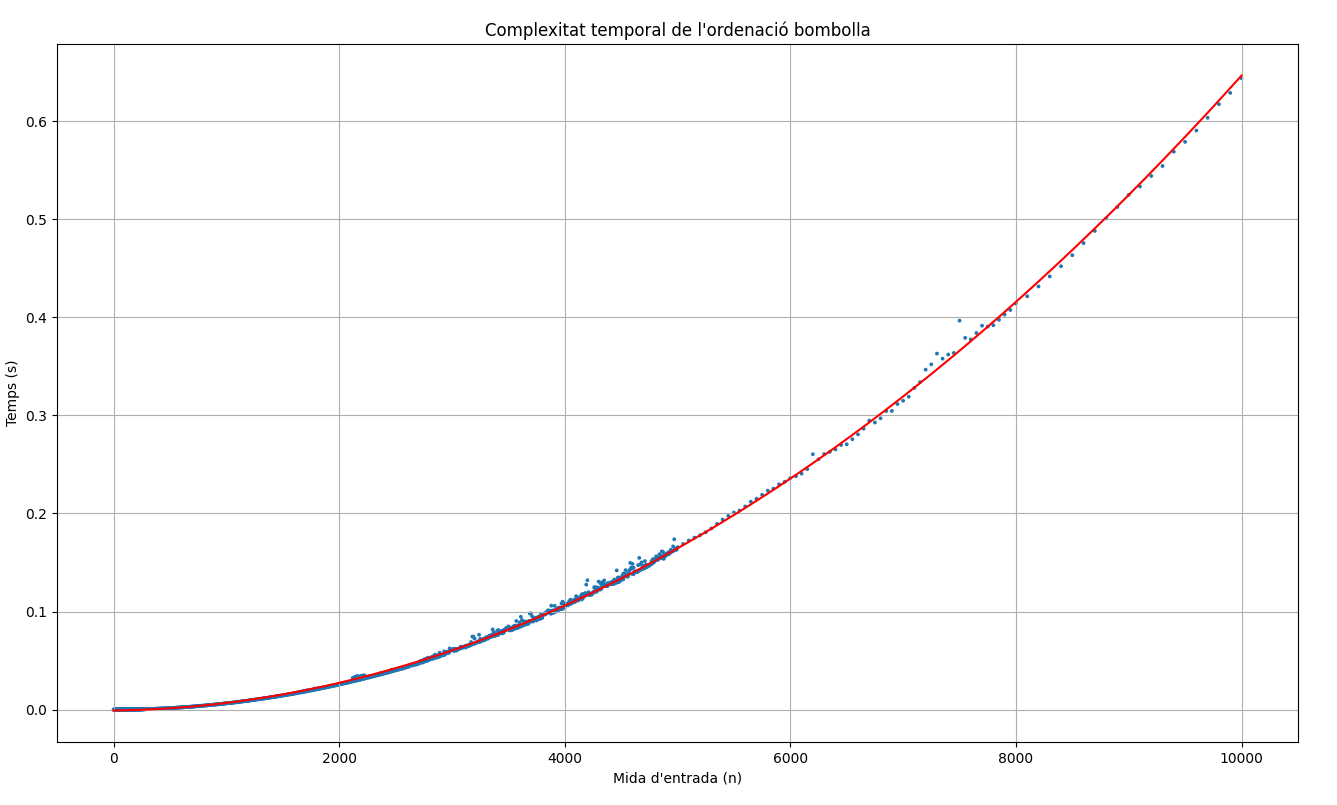
\includegraphics[width=1\textwidth]{capitols/figures/bombollascaterline.png}
    \caption[Gràfic de dispersió de l'ordenació bombolla amb la corba de regressió $f(x) = 6.33 \cdot 10^{-9} x^2 + 1.4 \cdot 10^{-6} x - 0.0008552$.]{Gràfic de dispersió de l'ordenació bombolla amb la corba de regressió $f(x) = 6.33 \cdot 10^{-9} x^2 + 1.4 \cdot 10^{-6} x - 0.0008552$. Font: elaboració pròpia.}
    \label{fig:my_label}
\end{figure}

% \vspace{-18pt}

Podem veure clarament que la forma que té el gràfic de la figura 3.10 s'assembla molt a la funció quadràtica. A més, encaixa perfectament amb la corba de regressió polinòmica.

\begin{figure}[H]
    \centering
    % \vspace{-18pt}
\begin{tikzpicture}
\centering
\begin{axis}[xmin=0, xmax=25, ymin=0, ymax=700, axis lines = middle, 
x label style={at={(axis description cs:0.5,-0.1)},anchor=north},
y label style={at={(axis description cs:-0.1,.5)},rotate=90,anchor=south},
xlabel={$n$ mida de l'entrada},
ylabel={nombre d'operacions},
style={thick}, 
compat=1.18, width=.4\textwidth, 
% legend style={nodes={scale=0.75, transform shape}}, 
legend pos=south east]
\addplot[color=vermellpral, domain=0:25, samples=150]{x^2};
% \addplot[color=verd, domain=0:10]{2*(x^2)};
\legend{$O(n^2)$, $O(2 \cdot n^2)$}
\end{axis}
\end{tikzpicture}
    \caption[Gràfic de complexitat quadràtica.]{Gràfic de complexitat quadràtica. Font: elaboració pròpia.}
    \label{fig:my_label}
\end{figure}

Per tant, amb l'estudi matemàtic i empíric hem arribat a la mateixa conclusió: l'ordenació bombolla té complexitat quadràtica.

\subsubsection{Anàlisi empíric de l'ordenació per barreja}
Aquest algoritme l'he executat 54.260 vegades. Ho he fet 10 vegades per cada mida d'entrada d'entre 10 i 30.000 en intervals de 10 unitats, de 30.050 a 100.000 en intervals de 50 unitats i de 100.100 a 200.000 en intervals de 100 unitats. També he reforçat amb més mostres les parts del gràfic que s'allunyaven més de la resta de mostres.

Finalment he obtingut el següent gràfic:
\begin{figure}[H]
    \centering
    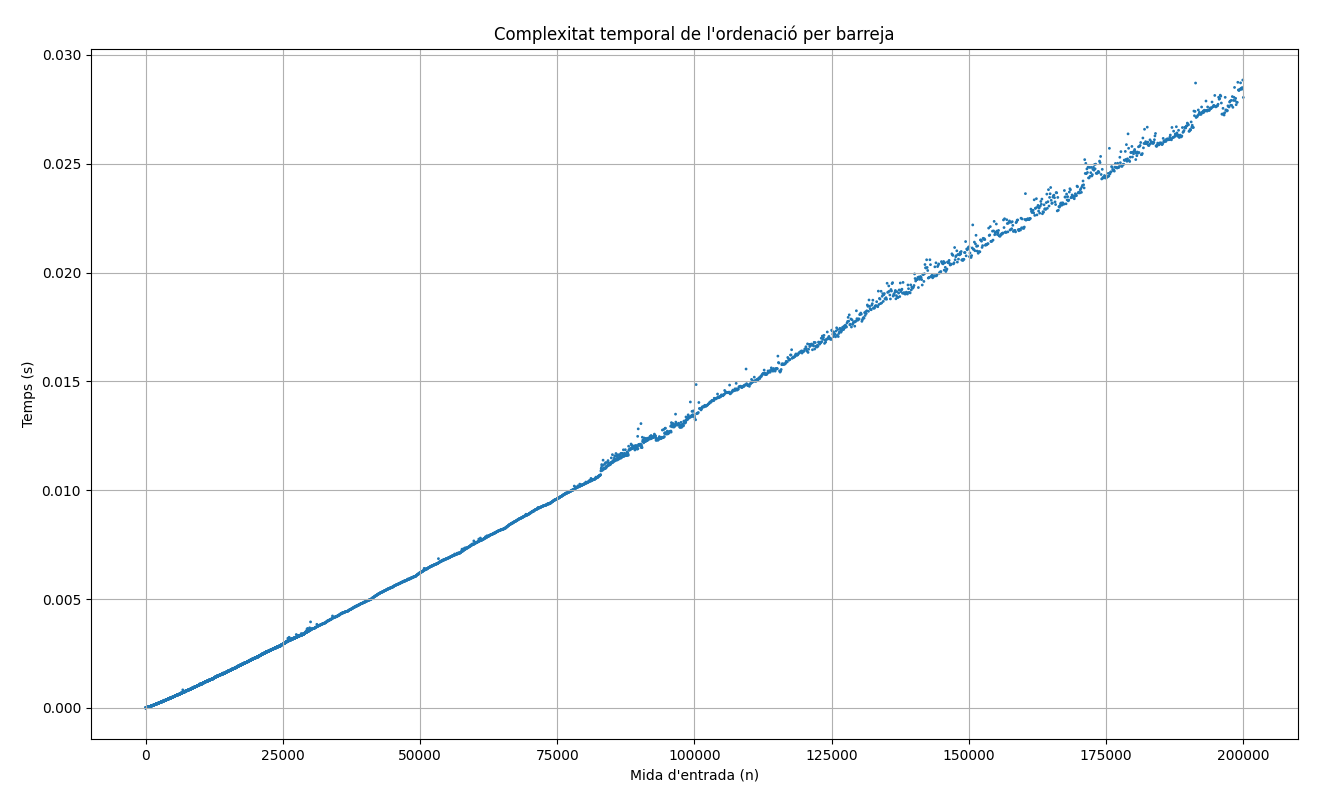
\includegraphics[width=1\textwidth]{capitols/figures/mergescatter.png}
    \caption[Gràfic de dispersió de l'ordenació per barreja.]{Gràfic de dispersió de l'ordenació per barreja. Font: elaboració pròpia.}
    \label{fig:my_label}
\end{figure}
\vspace{-18pt}
Sembla una recta així que podríem dibuixar al gràfic una recta de regressió lineal:
\begin{figure}[H]
    \centering
    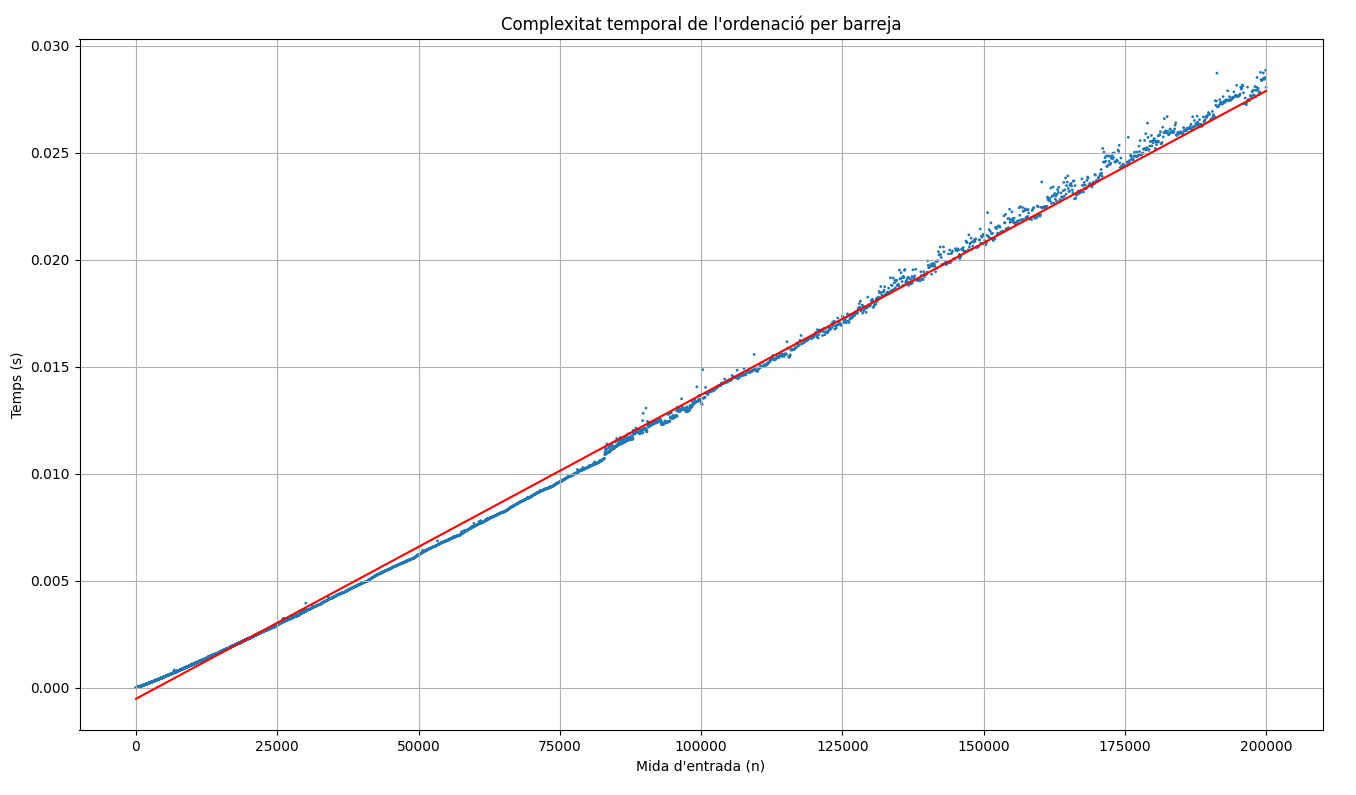
\includegraphics[width=1\textwidth]{capitols/figures/mergescaterline.png}
    \caption[Gràfic de dispersió de l'ordenació per barreja amb la recta de regressió lineal.]{Gràfic de dispersió de l'ordenació per barreja amb la recta de regressió lineal. Font: elaboració pròpia.}
    \label{fig:my_label}
\end{figure}

Si comparem la recta vermella amb les dades que hem obtingut, podem veure que no acaba d'encaixar.

En l'anàlisi matemàtic hem arribat a la conclusió que aquest algoritme té complexitat $O(n \cdot \log_2{n})$. Així que podem comparar les figures 3.12 i 3.14.
\begin{figure}[H]
    \centering
    % \vspace{-18pt}
\begin{tikzpicture}
\centering
\begin{axis}[xmin=0, xmax=25, ymin=0, ymax=150, axis lines = middle, 
x label style={at={(axis description cs:0.5,-0.1)},anchor=north},
y label style={at={(axis description cs:-0.1,.5)},rotate=90,anchor=south},
xlabel={$n$ mida de l'entrada},
ylabel={nombre d'operacions},
style={thick}, 
compat=1.18, width=.4\textwidth, 
legend style={nodes={scale=0.8, transform shape}}, 
legend pos=south east]
\addplot[color=vermellpral, domain=0:25, samples=150]{x*log2(x)};
% \addplot[color=verd, domain=0:10]{2*(x^2)};
\legend{$O(n \cdot \log_2{n})$}
\end{axis}
\end{tikzpicture}
    \caption[Gràfic de complexitat $O(n \cdot \log_2{n})$.]{Gràfic de complexitat $O(n \cdot \log_2{n})$. Font: elaboració pròpia.}
    \label{fig:my_label}
\end{figure}

Podem veure com els gràfics s'assemblen, encara que no tant com en els altres tres algoritmes. 


En aquest gràfic i el de la cerca dicotòmica no he trobat la recta de regressió, ja que és més complicat quan les funcions són logarítmiques.

\chapter{\LaTeX}
Finalment, he escrit tot aquest treball programant-ho en \LaTeX \space i utilitzant l'editor overleaf. 

En aquest enllaç hi ha tots els fitxers del document: (reposetori a github amb els documents) o escanejant el codi QR de la figura 4.1:

\chapter{Conclusions}
\input{capitols/conclusió}

\chapter{Referències}
[1] “Sections and chapters.” Consulta 1 d’abril 2022. \url{https://es.overleaf.com/learn/latex/Sections_and_chapters}

[2] Admin. “Your Guide to Fancy Chapters in LaTeX.” LaTeX-Tutorial.Com (blog). Consulta 12 d’abril 2022. \url{https://latex-tutorial.com/fancy-chapters-latex/}

[3] TeX - LaTeX Stack Exchange. “Glenn Fncychap + Color of the Box.” Consulta 13 d’abril 2022. \url{https://tex.stackexchange.com/questions/405297/glenn-fncychap-color-of- \\ the-box} 

[4] “Using Colours in LaTeX.” Consulta 13 d’abril 2022. \url{https://www.overleaf.com/learn/latex/Using_colours_in_LaTeX}

[5] “¿Qué Es Un Algoritmo y Qué Es Un Programa?” Consulta 18 de juny 2022. \url{http://www.edu4java.com/es/conceptos/que-es-un-algoritmo-que-es-un-programa.html}

[6] “Lista Completa de Símbolos En LaTeX | Manualdelatex.Com.” Consulta 18 de juny 2022. \url{https://manualdelatex.com/simbolos#chapter8}

[7] --“ZoteroBib: Fast, Free Bibliography Generator - MLA, APA, Chicago, Harvard Citations.” Consulta 18 de juny 2022.   \url{https://zbib.org/#}

[8] ¿Qué Es Eso Del Problema P versus NP? Consulta 22 de juny 2022. \url{https://www.youtube.com/watch?v=UR2oDYZ-Sao}

[9] freeCodeCamp.org. “Beginners Guide to Big O Notation,”. Consulta 23 de juny 2022. \url{https://www.freecodecamp.org/news/my-first-foray-into-technology-c5b6e83fe8f1/}

[10] Mejia, Adrian. “How to Find Time Complexity of an Algorithm?” Adrian Mejia Blog. Consulta 23 de juny 2022. \href{https://adrianmejia.com/how-to-find-time-complexity-of-an-algorithm-code-big-o-notation/}{\nolinkurl{https://adrianmejia.com/how-to-find-time-complexity-of-an- \\ algorithm-code-big-o-notation/}}

[11] Roura, Salvador. «Eficiència d’algorismes». UPC. Consulta 23 de juny 2022. \url{https://www.cs.upc.edu/~roura/eficiencia.pdf}

[12] Big O Notation - Full Course. Consulta 6 de juliol 2022. \url{https://www.youtube.com/watch?v=Mo4vesaut8g}

[13] arvindpdmn, dineshpathak. “Algorithmic Complexity.” Consulta 7 de juliol 2022. \url{https://devopedia.org/algorithmic-complexity}

[14] “Real-World Example of Exponential Time Complexity.” Forum post. Stack Overflow, Consulta 7 de juliol 2022. \url{https://stackoverflow.com/q/7055652}

[15] Lovett, Pamela. “Big-O Notation: A Simple Explanation with Examples.” Consulta 7 de juliol 2022. \href{https://betterprogramming.pub/big-o-notation-a-simple-explanation-with-examples-a56347d1daca}{\nolinkurl{https://betterprogramming.pub/big-o-notation-a-simple-explanation- \\ with-examples-a56347d1daca}}

[16] “Hide an Entry from Toc in Latex.” Forum post. Stack Overflow. Consulta 12 de juliol 2022. \url{https://stackoverflow.com/q/2785260}

[17] Alraja, Humam Abo. “Logarithms & Exponents in Complexity Analysis.” Consulta 15 de juliol 2022. \href{https://towardsdatascience.com/logarithms-exponents-in-complexity-analysis-b8071979e847}{\nolinkurl{https://towardsdatascience.com/logarithms-exponents-in-complexity- \\ analysis-b8071979e847}}

[18] MIT. “Big O notation”.  Consulta 24 de juliol 2022. \url{https://web.mit.edu/16.070/www/lecture/big_o.pdf}

[19] GeeksforGeeks. “Bubble Sort Algorithm,” Consulta 24 de juliol 2022. \url{https://www.geeksforgeeks.org/bubble-sort/}



\chapter{Annex}
\section{Una solució al sudoku amb gràfics}
El programa està en aquest enllaç: \url{https://github.com/JordinaGR/sudoku} o escanejant el codi de la figura 7.1.
\begin{figure}[H]
    \centering
    
\includegraphics[width=.15\textwidth]{capitols/figures/qr2.png}
    \caption[Programa que resol els sudokus.]{Programa que resol els sudokus. Font: elaboració pròpia.}
    \label{fig:my_label}
\end{figure}

\section{Implementació de la cerca lineal}
\begin{figure}[H]
    \begin{minted}[
    frame=lines,
    framesep=2mm,
    baselinestretch=1.2,
    bgcolor=LightGray,
    fontsize=\footnotesize,
    linenos
    ]{c++}
    // Implementació en c++
    
    #include<bits/stdc++.h>
    using namespace std;

    int main(){
    	int n, k; cin >> n >> k;
    	int ans = -1;
    	
    	for (int i = 0; i < n; i++){
    		int x; cin >> x;
    		if (x == k) ans = i;
    	}
    	
    	cout << ans << endl;
    	
    }
    \end{minted}
    \caption[Implementació de cerca lineal.]{Implementació de cerca lineal en c++. Font: elaboració pròpia.}
    \label{Figura}
\end{figure}%
\begin{figure}[H]
    \begin{minted}[
    frame=lines,
    framesep=2mm,
    baselinestretch=1.2,
    bgcolor=LightGray,
    fontsize=\footnotesize,
    linenos
    ]{python}
    # Implementació en python
        
    n, k = map(int, input().split())
    ans = -1
    array = list(map(int, input().strip().split()))
    
    for i in range(n):
        if array[i] == k:
            ans = i
    
    print(ans)
    \end{minted}
    \caption[Implementació de cerca lineal.]{Implementació de cerca lineal en python. Font: elaboració pròpia.}
    \label{Figura}
\end{figure}

\section{Implementació de la cerca dicotòmica}
\begin{figure}[H]
    \begin{minted}[
    frame=lines,
    framesep=2mm,
    baselinestretch=1.2,
    bgcolor=LightGray,
    fontsize=\footnotesize,
    linenos
    ]{c++}
    // Implementació en c++
    #include <bits/stdc++.h>
    using namespace std;
    
    int binary(int l, int r, int k, vector<int> v){
        while (l <= r){
            int mid = (l+r)/2;
    
            if (v[mid] == k) return mid;
            else if (v[mid] > k) {
                r = mid-1;
            } else if (v[mid] < k) {
                l = mid+1;
            }
        }
        return -1;
    }
    int main(){
    
        int n, k; cin >> n >> k;
        vector<int> v(n);
        for (int i = 0; i < n; i++) cin >> v[i];
    
        int x = binary(0, n-1, k, v);
    
        cout << x << endl;
    }
    \end{minted}
    \caption[Implementació de la cerca dicotòmica en c++.]{Implementació de la cerca dicotòmica en c++. Font: elaboració pròpia.}
    \label{Figura}
\end{figure}
\begin{figure}[H]
    \begin{minted}[
    frame=lines,
    framesep=2mm,
    baselinestretch=1.2,
    bgcolor=LightGray,
    fontsize=\footnotesize,
    linenos
    ]{python}
    # Implementació en python
    def binary(l, r, arr):
        while l <= r:
            mid = (l+r) // 2
    
            if arr[mid] == k:
                return mid
            elif arr[mid] > k:
                r = mid-1
            elif arr[mid] < k:
                l = mid+1
    
        return -1
        
    n, k = map(int, input().split())
    array = list(map(int, input().strip().split()))
    
    x = binary(0, n-1, array)
    
    print(x)
    \end{minted}
    \caption[Implementació de la cerca dicotòmica en python.]{Implementació de la cerca dicotòmica en python. Font: elaboració pròpia.}
    \label{Figura}
\end{figure}

\section{Implementació de l'ordenació de bombolla}
\begin{figure}[H]
    \begin{minted}[
    frame=lines,
    framesep=2mm,
    baselinestretch=1.2,
    bgcolor=LightGray,
    fontsize=\footnotesize,
    linenos
    ]{c++}
    // Implementació en c++
    #include <bits/stdc++.h>
    using namespace std;
    
    int main(){
        int n; cin >> n;
        vector<int> v(n);
        for (int i = 0; i < n; i++){
            cin >> v[i];
        }
        for (int i = 0; i < n; i++){
            for (int j = 0; j < n-1; j++){
                if (v[j] > v[j+1]){
                    int tmp = v[j];
                    v[j] = v[j+1];
                    v[j+1] = tmp;
                }
            }
        }
        for (auto x : v){
            cout << x << ' ';
        } cout << endl;
    }
    \end{minted}
    \caption[Implementació de l'ordenació de bombolla en c++.]{Implementació de l'ordenació de bombolla en c++. Font: elaboració pròpia.}
    \label{Figura}
\end{figure}
\begin{figure}[H]
    \begin{minted}[
    frame=lines,
    framesep=2mm,
    baselinestretch=1.2,
    bgcolor=LightGray,
    fontsize=\footnotesize,
    linenos
    ]{python}
    # Implementació en python
    n = int(input())
    arr = list(map(int, input().strip().split()))
    
    for i in range(n):
        for j in range(0, n-1):
            if arr[j] > arr[j+1]:
                arr[j], arr[j+1] = arr[j+1], arr[j]
    
    print(*arr)
    \end{minted}
    \caption[Implementació de l'ordenació de bombolla en python.]{Implementació de l'ordenació de bombolla en python. Font: elaboració pròpia.}
    \label{Figura}
\end{figure}

\section{Implementació de l'ordenació per barreja}

\begin{longlisting}
    \begin{minted}[
    frame=lines,
    framesep=2mm,
    baselinestretch=1.2,
    bgcolor=LightGray,
    fontsize=\footnotesize,
    linenos
    ]{c++}
    // Implementació en c++
    
    #include <bits/stdc++.h>
    using namespace std;
    
    void merge(vector<int>& v, int l, int mid, int r){
        vector<int> vec;
        int i = l; int j = mid+1;
    
        while (i <= mid and j <= r){
            if (v[i] < v[j]){
                vec.push_back(v[i]);
                i++;
            } else {
                vec.push_back(v[j]);
                j++;
            }
        }
        while (i <= mid){
            vec.push_back(v[i]);
            i++;
        }
        while (j <= r){
            vec.push_back(v[j]);
            j++;
        }   
        int y = 0;
        for (int q = l; q <= r; q++){
            v[q] = vec[y];
            y++; 
        }
    }
    void mergeSort(vector<int>& v, int l, int r){
        if (l < r){
            int mid = (l+r) / 2;
            mergeSort(v, l, mid);
            mergeSort(v, mid+1, r);
    
            merge(v, l, mid, r);
        }
    }
    int main(){
        int n; cin >> n;
        vector<int> v(n);
        
        for (int i = 0; i < n; i++) cin >> v[i];
    
        mergeSort(v, 0, n-1);
    
        for (auto x : v){
            cout << x << ' ';
        } cout << endl;
    }
    \end{minted}
    \caption[Implementació de l'ordenació per barreja en c++.]{Implementació de l'ordenació per barreja en c++. Font: elaboració pròpia.}
    \label{Figura}
\end{longlisting}
\begin{longlisting}
    \begin{minted}[
    frame=lines,
    framesep=2mm,
    baselinestretch=1.2,
    bgcolor=LightGray,
    fontsize=\footnotesize,
    linenos
    ]{python}
    # Implementació en python
    
    def merge(arr, l, mid, r):
        b = []
        i, j = l, mid+1
    
        while i <= mid and j <= r:
            if arr[i] < arr[j]:
                b.append(arr[i])
                i += 1
            else:
                b.append(arr[j])
                j += 1
    
        while i <= mid:
            b.append(arr[i])
            i += 1
    
        while j <= r:
            b.append(arr[j])
            j += 1
    
        y = 0
        for q in range(l, r+1):
            arr[q] = b[y]
            y += 1
    
    def mergeSort(arr, l, r):
        if (l < r):
            mid = (l+r) // 2
            mergeSort(arr, l, mid)
            mergeSort(arr, mid+1, r)
    
            merge(arr, l, mid, r)
    
    
    n = int(input())
    arr = list(map(int, input().strip().split()))
    
    mergeSort(arr, 0, n-1)
    
    print(*arr)
    \end{minted}
    \caption[Implementació de l'ordenació per barreja en python.]{Implementació de l'ordenació per barreja en python. Font: elaboració pròpia.}
    \label{Figura}
\end{longlisting}


\end{document}